
\chapter{Desenvolvimento} \label{chapter-dev}

Este capítulo detalha o desenvolvimento do compilador escrito na linguagem Odin, que torna possível a transformação de equações em documentos \LaTeX{} em código GLSL. Cada etapa do processo é encapsulada em um pacote distinto, estruturado em diretórios conforme a \autoref{estrutura-de-pacotes}. O \texttt{lexer} corresponde à tokenização da linguagem, responsável por converter o texto em \textit{tokens} identificáveis. O \texttt{parser} realiza a análise sintática, construindo a estrutura gramatical do documento. O \texttt{walker} contém funções essenciais para visualização da árvore de sintaxe abstrata (AST) e checagem de tipos feita pelo \texttt{checker}, executando a travessia da árvore de forma ordenada para geração de código feita pelo pacote \texttt{emitter}. A arquitetura completa do compilador pode ser vista na \autoref{fig-estrutura-geral-compilador}.

\begin{figure}[!ht]
  \caption{\label{fig-estrutura-geral-compilador} \small Estrutura de geral da arquitetura do compilador.}
  \begin{center}
    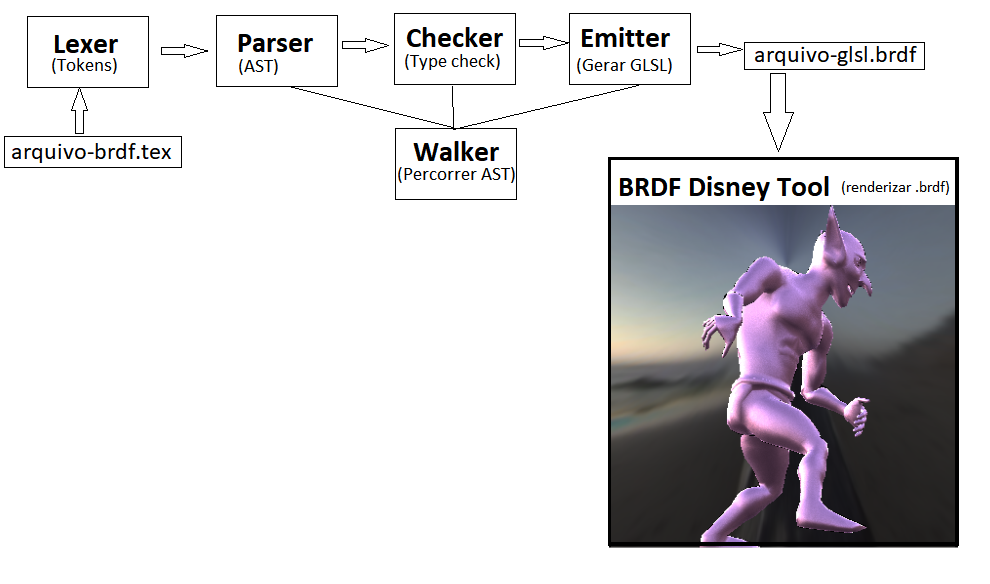
\includegraphics[scale=0.62]{./Imagens/estutura-geral-do-projeto.png}
  \end{center}
\end{figure}


\begin{figure}[!ht]
  \caption{\label{estrutura-de-pacotes} \small Estrutura de pacotes do compilador.}
  \begin{center}
    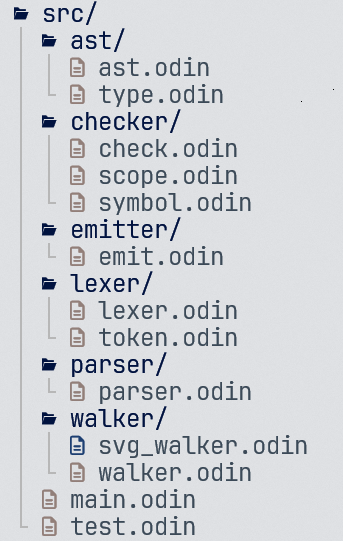
\includegraphics[scale=0.5]{./Imagens/package-structure.png}
  \end{center}
\end{figure}

No módulo \texttt{lexer}, explicado na \autoref{section-lexer}, foi implementada uma análise léxica manual inspirada em máquina de estados para tokenização do documento \LaTeX{}. Este processo converte a entrada textual em uma sequência de \textit{tokens}, preparando o as estruturas de dados para as próximas etapas de processamento.


Na \autoref{section-parser}, é discutido sobre o pacote \texttt{parser}, que utiliza gramática livre de contexto e a técnica de \textit{Pratt Parsing} para construir a árvore de sintaxe abstrata (AST). Essa abordagem possibilita uma representação hierárquica precisa das expressões matemáticas de BRDFs, capturando as nuances sintáticas e estruturais do documento original. A especificação da linguagem, apresentada no \autoref{grammar-ast-pt1} (parte 1) e no \autoref{grammar-ast-pt2} (parte 2), é definida na seção de análise sintática, juntamente com a precedência dos operadores prefixos e infixos.

O componente \texttt{walker}, discutido na \autoref{section-walker}, desempenha funções essenciais para a navegação e análise da AST. Suas funcionalidades incluem tanto a visualização da estrutura gerada quanto a preparação para verificações subsequentes por meio do pacote \texttt{checker}. O papel principal do \texttt{walker} é realizar a travessia dessa árvore de forma genérica, oferecendo suporte para decidir se a travessia deve continuar ou se é necessário retornar de um nó antes de alcançar os nós-folha. Além disso, o componente abstrai a forma de percorrer nós filhos de maneira uniforme, independentemente do tipo do nó pai.

No módulo \texttt{checker} (\autoref{section-checker}), foram implementadas as inferências de tipos e validações semânticas. Este componente garante a consistência das expressões matemáticas antes da geração de código, com o auxílio da tabela de símbolos (\autoref{subsection-symbols-scopes}), eliminando potenciais erros de modelagem. A saída dessa etapa deve estar apta para emitir código GLSL, com os símbolos organizados na ordem correta.

Por fim, o \texttt{emitter} utiliza a AST validada, a tabela de símbolos e os escopos para gerar código GLSL, transformando as expressões matemáticas de BRDFs contidas na AST em um \textit{shader} com toda implementação necessária para ser carregado na ferramenta de visualização Disney BRDF Explorer. Os resultados detalhados e os experimentos com a aplicação do compilador em BRDFs usadas na literatura podem ser consultados no \autoref{chapter.resultados}, onde é demonstrada a eficácia da ferramenta na tradução de diversos modelos de BRDFs. Esses experimentos também serviram como guia para a verificação da corretude da gramática durante seu desenvolvimento.



\section{Análise Léxica (\texttt{lexer})} \label{section-lexer}


Nesta etapa, é realizado o processo de tokenização de um subconjunto dos símbolos possíveis no ambiente de equação do \LaTeX{}, conforme comentado na \autoref{especificacao-linguagem}. A entrada desse processo são caracteres do arquivo fonte, enquanto a saída é uma sequência lógica desses caracteres, organizada em \textit{tokens}. O código responsável por essa funcionalidade  está contido no pacote \texttt{lexer}.

O processo de análise léxica realiza uma varredura completa no arquivo de entrada, caractere por caractere, para identificar e extrair os \textit{tokens}. Antes de iniciar essa extração, verificamos se o trecho analisado pertence a um ambiente de equação. Essa verificação é feita ao identificar a \textit{string} \verb|\begin{equation}|, que marca o início da extração de \textit{tokens}. Da mesma forma, a delimitação do ambiente se encerra com a \textit{string} \verb|\end{equation}|. Isso permite que o sistema ignore partes do arquivo que não pertencem ao ambiente de equação, como textos explicativos ou outros elementos presentes no mesmo arquivo \texttt{.tex}. Dessa forma, garantimos que a tokenização seja restrita às secções relevantes do código.

    
% Para fins de documentação e maior clareza, definimos uma lista estruturada de expressões regulares que descreve a geração dos \textit{tokens}, apresentada na \autoref{grammar-tokens}\footnote{Vale observar que a "gramática dos \textit{tokens}" não possui atributos típicos de gramáticas livres de contexto, como recursão, símbolo inicial ou lados direitos compostos por não-terminais. Assim, pode ser mais adequado considerá-la como uma lista estruturada de expressões regulares.}.
%
% O alfabeto dessa gramática é composto pelos caracteres do arquivo fonte. Apesar de ser chamada de gramática, ela se assemelha mais a um conjunto de expressões regulares que descrevem padrões utilizados para identificar os \textit{tokens}. A escolha do termo "gramática" reflete a intenção de estabelecer uma a sintaxe de descrição da gramatica que será usada na gramática da análise sintática, a qual faz uso de uma gramática livre de contexto (GLC) para construção da árvore de sintaxe abstrata. Internamente, a geração dos \textit{tokens} é implementada como a simulação de uma máquina de estados finitos, que segue os padrões definidos por essas expressões regulares.

    % Para fins de documentação e maior clareza, definimos uma gramática que descreve a geração dos \textit{tokens}, apresentada na \autoref{grammar-tokens}\footnote{essa gramatica está mais para uma lista}. O alfabeto dessa gramática é composto pelos caracteres do arquivo fonte. Apesar de documentar com uma gramática, a geração dos \textit{tokens} é implementada internamente de maneira semelhante à simulação de uma máquina de estados.

Na lista de expressões regulares (\autoref{grammar-tokens}), definimos os tipos de \textit{tokens}, onde o lado esquerdo do símbolo ``$=$'' corresponde ao tipo de \textit{token}, e o lado direito descreve sua expressão regular. Palavras em letras maiúsculas representam categorias de caracteres, como \texttt{DIGIT}, que denota qualquer dígito de 0 a 9, e \texttt{LETTER}, que cobre letras de \texttt{`a'} a \texttt{`z'}. Já palavras entre aspas simples correspondem a sequências literais de caracteres.

Além disso, utilizamos os seguintes símbolos na notação: ``$*$'' indica zero ou mais ocorrências do caractere especificado; ``$|$'' representa alternativas para a geração do mesmo tipo de \textit{token}; e ``$;$'' marca o fim da definição do tipo de \textit{token}.

%%%%%%%%%%%%%

O pacote inteiro de tokenização pode ser acessado por meio de uma única função, descrita no \autoref{function-lex}, escrita na linguagem \texttt{Odin}. Essa função, chamada \texttt{lex}, aceita uma lista de caracteres como entrada e retorna uma lista de estruturas do tipo \texttt{Token} (detalhado no \autoref{lexer-structs}). A estrutura \texttt{Token} possui três campos principais:

\begin{itemize}
    \item \texttt{kind}: identifica o tipo de \textit{token}, mapeando-o para uma dos tipos definidos no \autoref{grammar-tokens}.
    \item \texttt{text}: contém a \textit{string} correspondente ao \textit{token} gerado.
    \item \texttt{position}: uma instância do tipo \texttt{Position}, que registra a posição exata do \textit{token} no arquivo de origem.
\end{itemize}


\begin{codigo}[H]
        \caption{\small Função principal do Lexer. }
        \label{function-lex}
\begin{lstlisting}[language = c]
  
    lex :: proc(input: []u8) -> []Token
\end{lstlisting}
\end{codigo}



Durante a iteração sobre o \texttt{input}, o processo de tokenização mantém algumas variáveis de controle para monitorar o estado do fluxo de caracteres. Quebras de linha são contadas ao encontrar sequências como \verb|"\n"| ou \verb|"\n\r"|. É mantida a coluna atual que rastreia a posição horizontal do caractere em uma linha. O cursor é o índice que aponta para o caractere atualmente em processamento. Essas informações são usadas para preencher o campo \texttt{position} de cada \textit{token}. A estrutura \texttt{Position}, detalhada no \autoref{lexer-structs}, é essencial para garantir a precisão na geração de relatórios e rastreamento de erros.

\subsection{Reporte de Erros} \label{subsection-erros}

O sistema informação de erros, implementado nesta etapa, é utilizado por todos os pacotes do projeto. Essa funcionalidade assegura que erros sejam associados a posições específicas no arquivo de entrada, facilitando a depuração e correção. A assinatura da função de tratamento de erros, bem como suas possíveis variações, está documentada no \autoref{cod-function-errors}.

\begin{codigo}[H]
    \caption{\small Função de erro exposto pelo pacote \texttt{lexer}. }
        \label{cod-function-errors}
\begin{lstlisting}[language=C++]
error_from_pos :: proc(pos: Position, msg: string, args: ..any)
error_from_token :: proc(token: Token, msg: string, args: ..any);
\end{lstlisting}
\end{codigo}


Dada uma posição ou um \texttt{token}, é exibida uma mensagem (\texttt{msg}) diretamente no terminal, formatada para destacar visualmente o erro em vermelho. A formatação utiliza as informações do \texttt{token}, como o nome do arquivo, a linha, a coluna e o comprimento do \texttt{token} problemático, permitindo sublinhar precisamente onde o erro ocorreu. Isso proporciona maior clareza às mensagens de erro, como exemplificado no caso de erro semântico devido ao uso de identificadores não definidos (\autoref{error-undefined-symbol}).

Optou-se por apresentar nesta seção uma visão geral de alguns erros possíveis para demonstrar como o compilador os reporta visualmente, independentemente de serem léxicos, sintáticos ou semânticos. Essa abordagem evita sobrecarregar as seções de análise sintática e semântica com descrições ou imagens excessivas. Nas análises seguintes, os tipos de erro serão discutidos em suas etapas correspondentes. A seguir, são apresentados exemplos de erros possíveis:

\begin{enumerate}
   \item \textbf{Erros léxicos}: uso de palavras reservadas (\autoref{error-reserved-word}).
   
   \item \textbf{Erros sintáticos}: problemas de estrutura, como balanceamento incorreto de parênteses (\autoref{error-balanceamento}) e \textit{tokens} que não formam uma expressão matemática válida (\autoref{error-cant-make-expression}).
   
   \item \textbf{Erros semânticos}: envolvendo tipos incompatíveis (\autoref{error-incompatible-types}), símbolos não definidos (\autoref{error-undefined-symbol}) e redefinição de símbolos (\autoref{error-redefinition}).
\end{enumerate}


% Outros exemplos de erros seguem o mesmo padrão de exibição e incluem: tipos incompatíveis (\autoref{error-incompatible-types}), símbolos não definidos (\autoref{error-undefined-symbol}), balanceamento de parênteses (\autoref{error-balanceamento}), uso de palavras reservadas (\autoref{error-reserved-word}) .

\begin{figure}[H]
    \caption{\label{error-undefined-symbol} \small Erro ao tentar símbolo não definido.}
    \begin{center}
        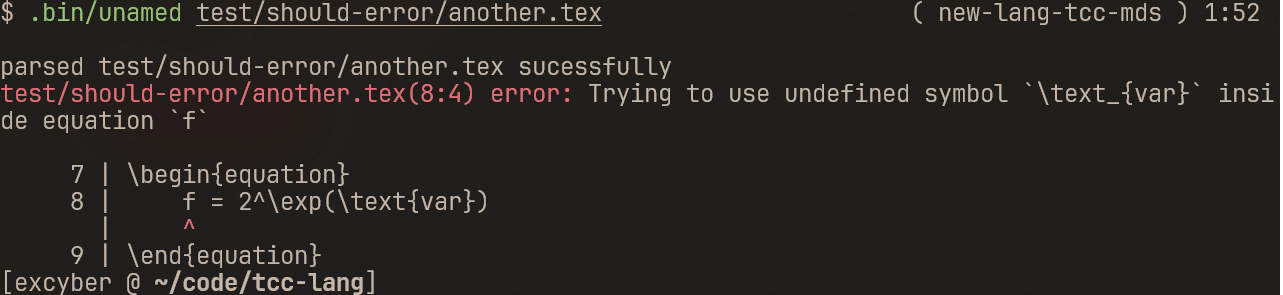
\includegraphics[scale=0.5]{./Imagens/error-undefined-symbol.png}
    \end{center}
\end{figure}

\begin{figure}[H]
    \caption{\label{error-incompatible-types} \small Erro de tipos incompatíveis.}
    \begin{center}
        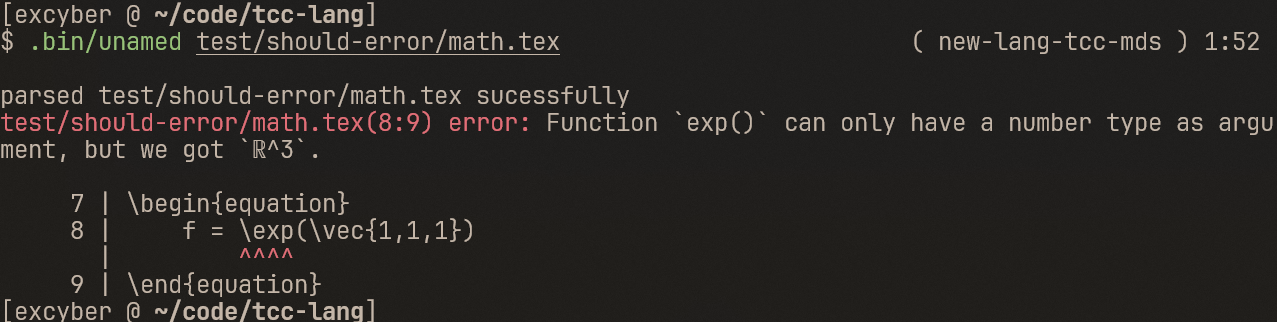
\includegraphics[scale=0.5]{./Imagens/error-incompatible-types.png}
    \end{center}
\end{figure}


\begin{figure}[H]
    \caption{\label{error-balanceamento} \small Erro de balanceamento de parênteses.}
    \begin{center}
        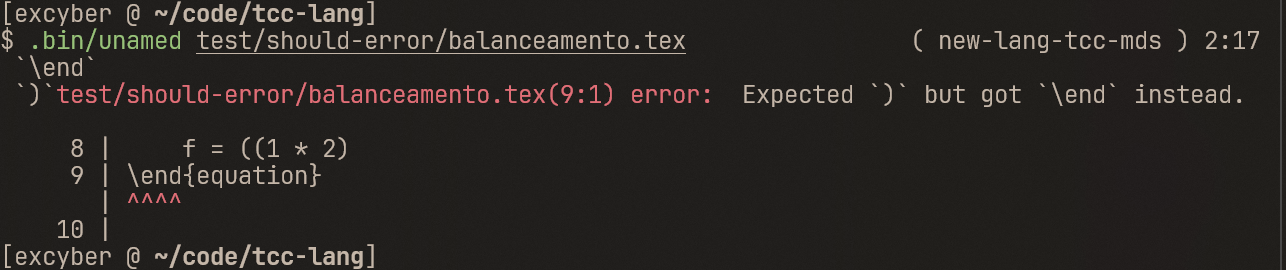
\includegraphics[scale=0.5]{./Imagens/error-balanceamento.png}
    \end{center}
\end{figure}

\begin{figure}[H]
    \caption{\label{error-reserved-word} \small Erro de uso incorreto de palavras reservadas.}
    \begin{center}
        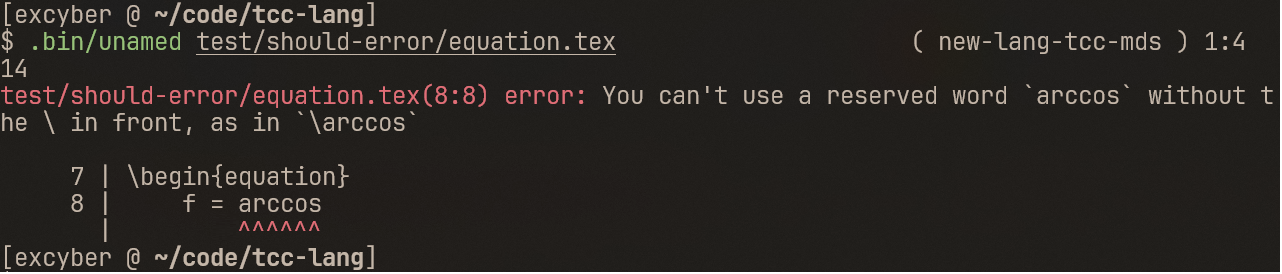
\includegraphics[scale=0.5]{./Imagens/error-reserved-word.png}
    \end{center}
\end{figure}


\begin{figure}[H]
    \caption{\label{error-cant-make-expression} \small Erro de \textit{token} incapaz de produzir expressão.}
    \begin{center}
        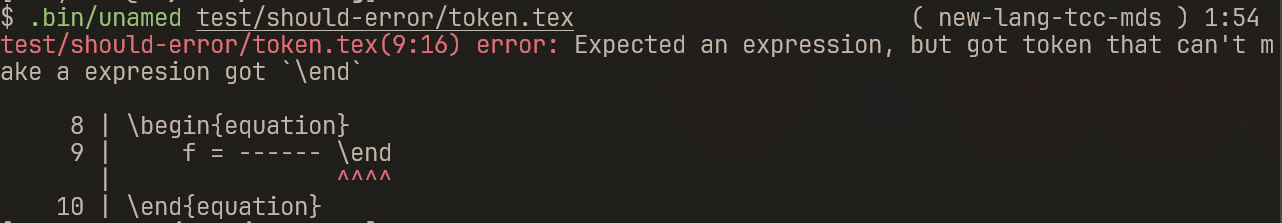
\includegraphics[scale=0.5]{./Imagens/error-cant-make-expression.png}
    \end{center}
\end{figure}

\begin{figure}[H]
    \caption{\label{error-redefinition} \small Erro de redefinição de símbolo.}
    \begin{center}
        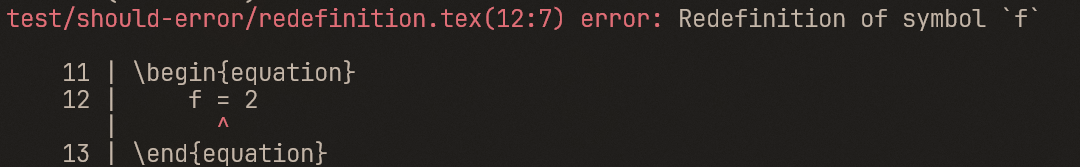
\includegraphics[scale=0.5]{./Imagens/error-redefinition.png}
    \end{center}
\end{figure}



\subsection{Classificação e Extração de Tokens}

Tokens simples, como aqueles compostos por um ou dois caracteres, são extraídos lendo-se o número correspondente de caracteres do \texttt{input}. Após a leitura, o \texttt{token} é construído e o laço continua para o próximo. Quando um caractere \texttt{\%} é encontrado, os caracteres subsequentes são ignorados até a próxima quebra de linha. Isso adiciona suporte a comentários no estilo \LaTeX{}.

Tokens mais complexos, como números, identificadores ou \textit{tokens} especiais, são extraídos com base em suas características. Números podem opcionalmente conter um ponto decimal, como em $1.0$. Já identificadores consistem em uma ou mais letras, opcionalmente prefixadas pelo símbolo \verb|\|.

A lista de expressões regulares de \textit{tokens} fornecida é intrinsecamente ambígua. Por exemplo, uma sequência como \verb|\frac| pode ser interpretada como um identificador comum ou como \verb"token_frac". Para resolver essa ambiguidade, criamos um dicionário que mapeia identificadores específicos para \textit{tokens} especiais (\autoref{map-special-identifiers}). Assim, se um identificador começar com o caractere \verb|\|, ele será verificado no dicionário e classificado como um \textit{token} especial, se apropriado.


\label{lexer-subexpression}
Identificadores não permitem números nem mesmo o caractere de sublinhado (\verb|_|). Isso ocorre porque, no analisador sintático, um nó do tipo identificador é modelado como um tipo recursivo, permitindo que identificadores sejam aninhados ao conter outros nós. Dessa forma, não é necessário permitir sublinhados diretamente no nível de token, o que possibilita a escrita de identificadores mais complexos, como \verb|\pi{n_1}| (renderizado em \LaTeX{} como $\pi_{n_1}$). Nesse caso, \verb|\pi| seria o primeiro \textit{token} do nó identificador, e sua subexpressão seria \verb|n_1| (renderizado como $n_1$), que, por sua vez, é o identificador \verb|n| com a subexpressão \verb|1|.


Adicionalmente, permitimos o uso da palavra-chave \verb|\text|, como em \verb|\text{id}|, para descrever identificadores. Essa palavra-chave é utilizada para incluir texto dentro do ambiente de equações em \LaTeX{}, que pode oferecer uma visualização mais clara de funções longas. Por exemplo, em vez de renderizar `\( normalize(x) \)', pode-se usar \verb|\text{normalize}(x)|, que será renderizado como `\( \text{normalize}(x) \)', tornando a expressão mais legível. Outro caso útil pode ser o \textit{token} `\( len \)', que pode ser visualmente confundido com a multiplicação entre \(l\), \(e\) e \(n\); usando \verb|\text{len}|, fica mais claro que `\(\text{len}\)' é um único \textit{token}, e não como uma multiplicação entre 3 outros \textit{tokens}. A extração do \textit{token} \verb|\text| segue um processo semelhante ao do suporte para \verb|\vec{id}|.

A enumeração que representa os tipos de \textit{tokens} pode ser consultada no \autoref{enum-token-kind}. Cada entrada dessa enumeração corresponde diretamente aos tipos de \textit{tokens} gerados pela lista de expressões regulares apresentada no \autoref{grammar-tokens}. Para facilitar a leitura, incluímos o símbolo correspondente à direita de cada entrada, indicado em comentários.

Com a etapa de tokenização concluída, é possível avançar para a análise sintática, onde é explorada a forma como os \textit{tokens} gerados são organizados em estruturas hierárquicas que formam a árvore sintática.

\begin{codigo}[H]
        \caption{\small Estruturas do Lexer. }
        \label{lexer-structs}
\begin{lstlisting}[language=C++]

Token :: struct {
    kind: Token_Kind,
    val: union{i64,f64},
    text: string,
    pos:  Position,
}

Position :: struct {
    file:   string,
    offset: i64,   // starting at 0, buffer offeset in file
    line:   i64,   // starting at 1, starting
    column: i64,   // starting at 1
    length: int    // how much chars foward
}
    
  \end{lstlisting}
\end{codigo}




\begin{codigo}[H]
    \caption{\small Gramática ilustrativa para \texttt{tokens}. }
        \label{grammar-tokens}
  \begin{lstlisting}[numbers=none, frame=none, language=haskell]

    token_number     = DIGIT DIGIT* '.' DIGIT DIGIT* | DIGIT DIGIT*;
    token_identifier = '\' LETTER LETTER* | LETTER LETTER*;
    token_cmpgreater = '>';
    token_cmpless    = '<';
    token_cmpequal   = '==';
    token_equal      = '=';
    token_mul        = '*' | '\cdot';
    token_cross      = '\times';
    token_div        = '/';
    token_plus       = '+';
    token_minus      = '-';
    token_caret      = '^';
    token_semicolon  = ';';
    token_comma      = ',';
    token_colon      = ':';
    token_question   = '?';
    token_bang       = '!';
    token_openparen  = '(';
    token_closeparen = ')';
    token_opencurly  = '{';
    token_closecurly = '}';
    token_tilde      = '~';
    token_underline  = '_'; --- Used for subexpresions
    token_arrow      = '->';
    token_begin      = '\begin';
    token_end        = '\end';
    token_frac       = '\frac';
    token_vec        = '\vec';
    token_omega      = '\omega';
    token_theta      = '\theta';
    token_phi        = '\phi';
    token_rho        = '\rho';
    token_alpha      = '\alpha';
    token_beta       = '\beta';
    token_sigma      = '\sigma';
    token_pi         = '\pi';
    token_epsilon    = '\epsilon';
    token_max        = '\max';
    token_min        = '\min';
    token_exp        = '\exp';
    token_tan        = '\tan';
    token_sin        = '\sin';
    token_cos        = '\cos';
    token_arctan     = '\arctan';
    token_arcsin     = '\arcsin';
    token_arccos     = '\arccos';
    token_sqrt       = '\sqrt';
    token_text       = '\text';
    token_eof        = EOF;
    
  \end{lstlisting}
\end{codigo}



\begin{codigo}[H]
\caption{\small Enumeração dos tipos de \texttt{tokens}. }
    \label{enum-token-kind}
\begin{lstlisting}[language = C++]
  Token_Kind :: enum {
    EOF           = 0,
    Number,
    Identifier,

    Equal,        // =
    Mul,          // * ou \cdot
    Cross,        // X
    Div,          // /
    Plus,         // +
    Minus,        // -
    Caret,        // ^
    Comma,        // ,
    Colon,        // :
    Question,     // ?
    Bang,         // !
    OpenParen,    // (
    CloseParen,   // )
    OpenCurly,    // {
    CloseCurly,   // }
    Tilde,        // ~
    Underline,    // _
    Arrow,        // ->

    Begin = 256,  // \begin
    End,          // \end

    Frac,         // \frac
    Vec,          // \vec

    Omega,        // \omega
    Theta,        // \theta
    Phi,          // \phi
    Rho,          // \rho
    Pi,           // \pi
    Epsilon,      // \epsilon
    Alpha,        // \alpha
    Beta,         // \beta
    Sigma,        // \sigma

    Max,          // \max
    Min,          // \min
    Exp,          // \exp
    Tan,          // \tan
    ArcTan,       // \arctan
    Sin,          // \sin
    ArcSin,       // \arcsin
    Cos,          // \cos
    ArcCos,       // \arccos
    Sqrt,         // \sqrt

    Text,         // \text
    Invalid
}

\end{lstlisting}
\end{codigo}

\begin{codigo}[H]
        \caption{\small Mapa de identificadores especiais. }
        \label{map-special-identifiers}
  \begin{lstlisting}[language=C++]

SPECIAL_WORDS := map[string]Token{
    "text"  = Token{text = "\\text",     kind =.Text},

    // Special
    "frac"   = Token{text = "\\frac",    kind =.Frac},
    "vec"    = Token{text = "\\vec",     kind =.Vec},
    "cdot"   = Token{text = "\\cdot",    kind =.Mul},
    "begin"  = Token{text = "\\begin",   kind =.Begin},
    "end"    = Token{text = "\\end",     kind =.End},
    "rho"    = Token{text = "\\rho",     kind =.Rho},
    "sqrt"   = Token{text = "\\sqrt",    kind =.Sqrt},
    "omega"  = Token{text = "\\omega",   kind =.Omega},

    // Cross product
    "times"  = Token{text = "\\times",   kind =.Cross},

    "max"    = Token{text = "\\max",     kind =.Max},
    "min"    = Token{text = "\\min",     kind =.Min},
    "exp"    = Token{text = "\\exp",     kind =.Exp},

    "cos"    = Token{text = "\\cos",     kind =.Cos},
    "sin"    = Token{text = "\\sin",     kind =.Sin},
    "tan"    = Token{text = "\\tan",     kind =.Tan},

    "arccos" = Token{text = "\\arccos",  kind =.ArcCos},
    "arcsin" = Token{text = "\\arcsin",  kind =.ArcSin},
    "arctan" = Token{text = "\\arctan",  kind =.ArcTan},

    "theta"  = Token{text = "\\theta",   kind =.Theta},
    "phi"    = Token{text = "\\phi",     kind =.Phi},

    "alpha"   = Token{text = "\\alpha",  kind =.Alpha},
    "beta"    = Token{text = "\\beta",   kind =.Beta},
    "sigma"   = Token{text = "\\sigma",  kind =.Sigma},
    "pi"      = Token{text = "\\pi",     kind =.Pi},
    "epsilon" = Token{text = "\\epsilon",kind =.Epsilon},
}

    
  \end{lstlisting}
\end{codigo}


\section{Análise Sintática, (\texttt{parser})} \label{section-parser}

O \textit{parser} para a linguagem subconjunto do ambiente \verb|equation| do \LaTeX{} foi desenvolvido utilizando o método de Pratt \textit{Parsing} na linguagem Odin. Neste contexto, denominamos esse subconjunto como \texttt{EquationLang}, que abrange todas as partes essenciais para a definição de BRDFs descritas em \autoref{especificacao-linguagem}, além de sua gramática documentada.

A implementação deste \textit{parser} adota o método de descida recursiva, no qual cada regra de produção da gramática possui uma função de análise correspondente. Este método foi escolhido por priorizar a clareza e simplicidade do código, complementados por comentários detalhados para facilitar a compreensão. A entrada do \textit{parser} consiste nos \textit{tokens} gerados na etapa de análise léxica.


\subsection{Parser}

Diferentemente dos \textit{parsers} tradicionais de descida recursiva, que frequentemente utilizam múltiplas chamadas de função aninhadas para tratar diferentes níveis de precedência, o \textit{parser} aqui implementado organiza as funções de análise de forma hierárquica, com base na precedência dos operadores. Essa abordagem é detalhada no \autoref{alg-pratt-parsing}, que descreve a lógica central para o \textit{parsing} de expressões.

%%%%%%%%%%%%%%%%
Pratt Parsing simplifica a análise sintática de expressões ao tratar precedência e associatividade dinamicamente, sem inflar a gramática. Na abordagem tradicional, precedências são fixadas por meio de várias regras de produção, desmontrado no \autoref{cod-regras-tradicionais}.

\begin{codigo}[htb]
    \caption{\small Regras tradicionais de precendecia por gramática. }
    \label{cod-regras-tradicionais}
\begin{lstlisting}[language=haskell, numbers=none, inputencoding=utf8]
    Expr               = LogicalOrExpr;
    LogicalOrExpr      = LogicalOrExpr      '||' LogicalAndExpr    | LogicalAndExpr;

    LogicalAndExpr     = LogicalAndExpr     '&&' EqualityExpr      | EqualityExpr;

    EqualityExpr       = EqualityExpr       '==' RelationalExpr    | RelationalExpr;   ---  Igualdade


    RelationalExpr     = RelationalExpr     '<' AdditiveExpr       | AdditiveExpr;     ---  Comparação

    AdditiveExpr       = AdditiveExpr       '+' MultiplicativeExpr | MultiplicativeExpr;

    MultiplicativeExpr = MultiplicativeExpr '*' PrimaryExpr        | PrimaryExpr;

    PrimaryExpr        = '(' Expr ')' | NUMBER | Identifier;  --- Expressões primárias

\end{lstlisting}
\end{codigo}


Isso torna a gramática mais longa, necessitando de mais regras que derivam outras regras antes de chegar a um símbolo do alfabeto da gramática. Na descrição recursiva, regras são o mesmo que funções, o que significa que os métodos recursivos tradicionais com muitos níveis de precedência fazem mais chamadas recursivas em código, gerando mais lentidão e complexidade na implementação da descrição recursiva a ser mantida. No Pratt Parsing, uma única regra é suficiente:
\verb`Expr = Expr ( '||' | '&&' | '==' | '<' | '+' | '*' ) Expr;`.

A precedência é definida em uma tabela (\autoref{tab-token-precedence}), e o \textit{parser} consulta essa tabela dinamicamente para decidir a ordem de avaliação com base no operador encontrado. Isso reduz a complexidade, facilita alterações e melhora a eficiência do \textit{parser}, resultando em um código mais simples, eficiente e flexível para incluir novos operadores.

Foi usado a notação similiar à original de Pratt \cite{pratt}, as funções \verb"parse_null_denotations" e \texttt{parse\_left\_denotations} desempenham papéis equivalentes às funções \texttt{token.prefixo} e \texttt{token.infixo}, respectivamente, como demonstrado no \autoref{alg1}. Além disso, a abordagem de descida recursiva (top-down) permite que cada regra de produção definida na gramática (\autoref{grammar-ast-pt1}) seja diretamente mapeada para um procedimento em código. Isso pode ser observado, por exemplo, na função de análise do nó \texttt{Start} da AST (\autoref{cod-parsing-start}), que reflete diretamente as regras de produção \texttt{start}, \texttt{decl}, e \texttt{decl\_equation\_begin\_end\_block} especificadas na gramática demonstrada no \autoref{grammar-ast-pt1}.

Do ponto de vista da interface oferecida pelo pacote \texttt{parser}, todo o processo de análise sintática é abstraído em uma única chamada de função (\autoref{cod-func-and-structs}). A função principal, \texttt{parse}, trabalha em conjunto com a estrutura \texttt{Parser} para realizar a análise.

\begin{codigo}[H]
  \caption{\small Parsing de expressão em código Odin.}
        \label{alg-pratt-parsing}
  \begin{lstlisting}[language=C]


parse_expr :: proc(prec_prev: i64) -> ^Expr {
    /* expressions that takes nothing (null) as left operand */
    left := parse_null_denotations()
    /*
    . if current token is left associative or current token has higher precedence
    . than previous precedence then stay in the loop, effectively creating a left leaning
    . sub-tree, else, we recurse to create a right leaning sub-tree.
    */
    for precedence(peek()) > prec_prev + associativity(peek())  {
        /* expressions that needs a left operand such as postfix, mixfix, and infix operator */
        left = parse_left_denotations(left)
    }
    return left
}


  \end{lstlisting}
\end{codigo}

\begin{codigo}[htb]
        \caption{\small Estruturas e Funções do Parser. }
        \label{cod-func-and-structs}
  \begin{lstlisting}[language = C]
Parser :: struct {
    tokens:      []Token,
    cursor:      i64,
    error_count: int,
}

parse :: proc(using p: ^Parser) -> ^ast.Start {
    return parse_start(p)
}
  \end{lstlisting}
\end{codigo}

\begin{codigo}[htb]
    \caption{\small \textit{Parsing} do nó \texttt{Start}. }
        \label{cod-parsing-start}
  \begin{lstlisting}[language=C++]
parse_start :: proc(using p: ^Parser) -> ^ast.Start {
    node := ast.new(ast.Start)
    decls := [dynamic]^ast.Decl{}

    for peek(p).kind != .EOF {
        decl := parse_equation_begin_end_block(p)
        append(&decls, decl)
    }
    node.eof = next(p, Token_Kind.EOF)
    node.decls = decls[:]
    return node
}
    
  \end{lstlisting}
\end{codigo}



\subsection{Gramática}

Para formalizar a gramática da linguagem de entrada (\texttt{EquationLang}), estabelecemos regras detalhadas nos \autoref{grammar-ast-pt1} e \autoref{grammar-ast-pt2}. O \autoref{code-gramatica} apresenta um exemplo de código-fonte válido nesta linguagem, cuja renderização correspondente em \LaTeX{} é ilustrada em \autoref{code-gramatica-rendered}.

\label{code-gramatica-rendered} \begin{subequations}
\begin{equation}
    \rho_{d} = \vec{0.3,0.3,0.3}
\end{equation}
\begin{equation}
    \rho_{s} = \vec{0.0,0.2,1.0}*20
\end{equation}
\begin{equation}
f = \frac{\rho_{d}}{\pi} + \frac{\rho_{s}}{8*\pi} *
\frac{({\vec{n}}\cdot{\vec{h}})}
{({\vec{\omega_{o}}}\cdot{\vec{h}}) *
\max(({\vec{n}}\cdot{\vec{\omega_{i}}}),
({\vec{n}}\cdot{\vec{\omega_{o}}}))}
\end{equation}
\end{subequations}


\begin{codigo}[htb]
        \caption{\small Exemplo código escrito na linguagem \texttt{EquationLang}. }
        \label{code-gramatica}
\begin{lstlisting}[language=tex, frame=none]
\begin{equation}
    \rho_{d} = \vec{0.3,0.3,0.3}
\end{equation}

\begin{equation}
    \rho_{s} = \vec{0.0,0.2,1.0}*20
\end{equation}

\begin{equation}
f = \frac{\rho_{d}}{\pi} + \frac{\rho_{s}}{8*\pi} *
\frac{({\vec{n}}\cdot{\vec{h}})}
{({\vec{\omega_{o}}}\cdot{\vec{h}}) *
\max(({\vec{n}}\cdot{\vec{\omega_{i}}}),
({\vec{n}}\cdot{\vec{\omega_{o}}}))}
\end{equation}

\end{lstlisting}
\end{codigo}

\begin{codigo}[H]
        \caption{\small Gramática para \texttt{EquantionLang} parte 1.}
        \label{grammar-ast-pt1}
\begin{lstlisting}[language=haskell, numbers=none, inputencoding=utf8]
    start  = decl* token_eof;

    decl = decl_equation_begin_end_block;

    decl_equation_begin_end_block =
        token_begin token_opencurly 'equation' token_closecurly
        decl_equation
        token_end token_opencurly 'equation' token_closecurly;

    decl_equation = field;

    field = expr token_equal expr;

    expr = expr_identifier
        | expr_number
        | expr_vector_literal
        | expr_grouped
        | expr_prefix
        | expr_infix
        | expr_postfix
        --- Ressalto que `function_call` e `function_definition` tem a mesma construção.
        --- Apenas diferenciamos pela posição que aparecer, se à esquerda ou à direta de '=' da regra `field`.
        --- por exemplo `a = f(1)`, `f(1)` é uma chamada de função
        --- Já `f(x) = 1` é uma definição de função
        | expr_function_call
        | expr_function_definition
        | token_opencurly expr token_closecurly
    ;

    expr_identifier =
        --- Ex: `\text{id}`
        token_text token_opencurly expr_identifier token_closecurly
        --- Ex: `\vec{id}`
        token_vec token_opencurly expr_identifier token_closecurly
        --- Ex: `id_n`
        | expr_identifier token_underline expr_identifier
        --- Ex: `id_2`
        | expr_identifier token_underline token_number
        --- Ex: `id_{n+1}`
        | expr_identifier token_underline token_opencurly expr token_closecurly
        --- Token especiais como \phi ou \alpha
        | token_identifier
        | token_omega
        | token_theta   | token_phi
        | token_rho     | token_alpha
        | token_beta    | token_sigma
        | token_pi      | token_epsilon
        | token_max     | token_min
    ;

\end{lstlisting}
\end{codigo}

\begin{codigo}[H]
        \caption{\small Gramática para \texttt{EquantionLang} parte 2.}
        \label{grammar-ast-pt2}
\begin{lstlisting}[language=haskell, numbers=none, inputencoding=utf8]
    expr_number = token_number;

    expr_vector_literal = token_vec
        --- Ex: `\vec{1, 1, 1}`
        token_opencurly
        (expr_number token_comma)* expr_number
        token_closecurly
    ;

    expr_grouped = token_openparen expr token_closeparen;

    expr_prefix =
        (token_sqrt | token_exp | token_tan| token_cos | token_sin | token_arctan | token_arccos | token_arcsin | token_minus | token_plus) expr
    ;

    expr_infix = token_frac
        token_opencurly expr token_closecurly
        token_opencurly expr token_closecurly
        | expr token_plus     expr
        | expr token_minus    expr
        | expr token_mul      expr
        | expr token_cross    expr
        | expr token_cmpequal expr
        | expr token_div      expr
        | expr token_caret    expr
    ;

    expr_postfix = expr token_bang;

    expr_function_call = expr token_openparen
        (expr token_comma)* expr
        token_closeparen
    ;

    --- Mesmo que expr_function_call, em etapas posteriores é decidido qual tipo realmente é.
    expr_function_definition = expr token_openparen
        (expr token_comma)* expr
        token_closeparen
    ;
\end{lstlisting}
\end{codigo}

Na definição da gramática (\autoref{grammar-ast-pt1}), adotamos a notação sintática previamente estabelecida na \autoref{section-lexer}, com o adicional que sequências de três hífens ("\verb"---"") representam comentários para o leitor, sem impactar a definição gramatical.

A gramática definida nesta seção abrange regras para expressões, atribuições, agrupamento, literais numéricos e vetores, chamadas de funções, definições de funções e diversos operadores, como \texttt{expr\_prefix} e \texttt{expr\_infix}. O objetivo é fornecer uma linguagem capaz de expressar a sintaxe necessária para definições de BRDFs em \LaTeX{}. 

A tabela de operadores (\autoref{tab-token-precedence}) usada no Pratt Parsing é representada pela função \texttt{precedence\_from\_token}, que mapeia um token para um valor inteiro que representa sua precedência: quanto maior o valor, maior a precedência do operador. É importante observar que alguns tokens podem ser usados tanto como prefixos quanto como infixos, dependendo do contexto. Por exemplo, o token \texttt{(} pode ser um prefixo em uma expressão de agrupamento, como em \textbf{(}$2*3$\textbf{)}, mas também pode ser infixo em uma chamada de função, como em $f$\textbf{(}$x$\textbf{)}. O mesmo comportamento ocorre com o token \texttt{-}, que pode atuar como operador prefixo de negação ou infixo para subtração.


\begin{table}[h!]
\centering
\begin{tabular}{|l|c|c|}
\hline
\textbf{Tipo de Token} & \textbf{Prefixo} & \textbf{Precedência}\\ \hline
\texttt{+}            & Sim              & 25                   \\ \hline
\texttt{-}            & Sim              & 25                   \\ \hline
\texttt{(}            & Sim              & 100                  \\ \hline
\texttt{:}            & Sim              & 100                  \\ \hline
\texttt{*}            & Sim              & 100                  \\ \hline
% \texttt{\textasciitilde} & Sim              & 200               \\ \hline
\texttt{!}            & Sim              & 300                  \\ \hline
\texttt{(}            & Não              & 500                  \\ \hline
\texttt{>}            & Não              & 5                    \\ \hline
\texttt{<}            & Não              & 5                    \\ \hline
\texttt{+}            & Não              & 10                   \\ \hline
\texttt{-}            & Não              & 10                   \\ \hline
$\times$              & Não              & 20                   \\ \hline
\texttt{*}            & Não              & 20                   \\ \hline
\texttt{/}            & Não              & 20                   \\ \hline
\texttt{\textasciicircum} & Não           & 30                  \\ \hline
\texttt{!}            & Não              & 400                  \\ \hline
\end{tabular}
\caption{Tabela de Precedência dos Tokens}
\label{tab-token-precedence}
\end{table}


\subsubsection{Estrutura da Árvore de Sintaxe}
Nesta seção, apresentamos os tipos de nós que compõem a árvore de sintaxe abstrata (AST), utilizada no compilador da linguagem \texttt{EquationLang}. A estrutura da AST é formada por diversos tipos de nós que capturam os diferentes elementos da sintaxe da linguagem. Diferente da gramática definida no \autoref{lst-gramatica}, os nós aqui são representados em nível de código. Vale ressaltar que o nó \texttt{Expr}, o mais genérico, possui um campo adicional \texttt{ty\_inferred} do tipo \texttt{Type}. Esse campo será preenchido durante a etapa de análise semântica e utilizado na geração de código. A seguir, listamos a representação semântica de cada nó, detalhando os campos que compõem cada um deles.

@@Fix this
\begin{itemize}
\item \textbf{Node}: Estrutura base para todos os nós da AST.
      \textbf{Campos:}
      \texttt{kind} (\texttt{typeid}), guarda um número que indica qual o tipo do nó.

\item \textbf{Expr}: Representa expressões de forma geral.
      \textbf{Campos:}
      \texttt{expr\_derived} e \texttt{ty\_inferred} (\texttt{Type})

\item \textbf{Decl}: Representa genericamente declarações.

\item \textbf{Start}: O nó raiz da AST.
      \textbf{Campos:}
      \texttt{decls} lista de \texttt{Decl}, \texttt{eof} (\texttt{Token}).

\item \textbf{Decl\_Equation}: representa uma equação.
      \textbf{Campos:}
      \texttt{field} referencia à uma instancia do nó (\texttt{Field}).

\item \textbf{Field}: Representa uma atribuição qualquer, usando o simbolo '='.
      \textbf{Campos:}
      \texttt{name} (\texttt{\^Expr}), \texttt{equals} (\texttt{Token}), \texttt{value} (\texttt{\^Expr}).

\item \textbf{Expr\_Identifier}: Representa identificadores.
      \textbf{Campos:}
      \texttt{identifier} (\texttt{Token}), \texttt{is\_vector} (\texttt{bool}),
      \texttt{sub\_expression} (\texttt{\^Expr}), \texttt{var} (\texttt{Maybe(string)}).

\item \textbf{Expr\_Number}: Representa literais numéricos.
      \textbf{Campos:}
      \texttt{number} (\texttt{Token}).

\item \textbf{Expr\_Vector\_Literal}: Representa vetores literais.
      \textbf{Campos:}
      \texttt{vec} (\texttt{Token}), \texttt{numbers} (\texttt{[]\^Expr\_Number}).

  \item \textbf{Expr\_Grouped}: representa expressões agrupadas, geralmente por \(\), mas é permitido agrupor por \{\}.
      \textbf{Campos:}
      \texttt{open} (\texttt{Token}), \texttt{expr} (\texttt{\^Expr}), \texttt{close} (\texttt{Token}).

  \item \textbf{Expr\_Prefix}: representa expressão com operator prefixo (ex: -3).
      \textbf{Campos:}
      \texttt{op} (\texttt{Token}), \texttt{right} (\texttt{\^Expr}).

  \item \textbf{Expr\_Infix}: representa expressões para operador infixo, isto é entre expressões, (ex: 3+3).
      \textbf{Campos:}
        \texttt{left} (pointeiro de \texttt{Expr}), \texttt{op} (\texttt{Token}), \texttt{right} (pointeiro de \texttt{Expr}).

\item \textbf{Expr\_Function\_Call}: representa chamadas de função.
      \textbf{Campos:}
      \texttt{left} (ponteiro de \texttt{Expr}), \texttt{open} (\texttt{Token}),
      \texttt{exprs} (lista de poteiros de \texttt{Expr}), \texttt{close} (\texttt{Token}).

\item \textbf{Expr\_Function\_Definition}: representa definições de funções.
      \textbf{Campos:}
      \texttt{name} (\texttt{Expr\_Identifier}), \texttt{open} (\texttt{Token}),
      \texttt{parameters} (lista de \texttt{Expr\_Identifier}), \texttt{close} (\texttt{Token}).
\end{itemize}




No \autoref{lexer-subexpression}, é comentado que o \textit{parser} é capaz de lidar com identificadores aninhados, como, por exemplo, \( x_{i_1} \) (\verb"x_{i_1}"). No \autoref{cod-expression-ident-recursive}, apresentamos como esses identificadores são criados recursivamente. O código mostrado faz parte de uma função maior, sendo um recorte de um \texttt{switch}\footnote{\texttt{switch} e \texttt{case} em Odin funcionam da mesma forma que na linguagem de programação \texttt{C}} sobre a enumeração descrita no \autoref{enum-token-kind}. Dentro desse \texttt{switch}, temos um \texttt{case} que reconhece tokens de identificador ou símbolos especiais (\( \omega, \theta, \phi, \rho, \alpha, \beta, \sigma, \pi, \epsilon \)). Ao fazer uma chamada recursiva à função \texttt{parse\_expr}, o \textit{parser} permite a inclusão de subíndices numéricos, subexpresões de identificadores ou até expressões binárias, como \( n+1 \) em \( f_{n+1} \).

Isso confere maior flexibilidade na hora de expressar funções e equações para descrever as BRDFs, sendo muito comum o uso de subíndices numéricos. Na etapa de geração de código, essa capacidade de distinguir identificadores com subíndices é crucial, pois permite tratar semânticamente tokens aparentemente iguais de maneira diferenciada. Por exemplo, embora o primeiro token seja \( f \), \( f_1 \) e \( f_2 \) são semanticamente distintos, permitindo uma distinção precisa entre símbolos com o mesmo nome base, mas com significados diferentes devido aos seus índices.
%%%%%


\begin{codigo}[htb]
    \caption{\small Parte do código de \textit{parsing} de expressão para identificadores. }
        \label{cod-expression-ident-recursive}
  \begin{lstlisting}[language = C]
    case .Identifier,
         .Omega,     // \omega
         .Theta,     // \theta
         .Phi,       // \phi
         .Rho,       // \rho
         .Alpha,     // \alpha
         .Beta,      // \beta
         .Sigma,     // \sigma
         .Pi,        // \pi
         .Epsilon,   // \epsilon
        node := ast.new(ast.Expr_Identifier)
        node.identifier = next(p)
        if peek(p).kind == Token_Kind('_') {
            next(p)
            if peek(p).kind == Token_Kind('{') {
                next(p, '{')
                node.sub_expression = parse_expr(p, prec)
                next(p, '}')
            } else {
                //
                // If we're not using `identifier_{ }` then, we only allow simple number or identifier
                //
                sub_node := ast.new(ast.Expr_Identifier)
                if peek(p).kind == .Number {
                    // We only allow number as sub expressions
                    sub_node.identifier = next_expects_kind(p, .Number)
                } else {
                    sub_node.identifier = next_expects_kind(p, .Identifier, ..SPECIAL_IDENTIFIERS[1:])
                }
                node.sub_expression = sub_node
            }
        }
    
  \end{lstlisting}
\end{codigo}


O \autoref{cod-expression-ident-recursive}, já apresentado, serve como exemplo para outras expressões recursivas, como expressões infixas (operações binárias). Para identificar o token atual, utilizamos a função \texttt{peek()}, que permite visualizar um ou dois tokens à frente e, com isso, decidir qual nó da AST (Árvore de Sintaxe Abstrata) deve ser construído. Após identificar o token, calculamos a variável \texttt{prec}, que indica a precedência do token atual. Com base nessa precedência, fazemos uma ou mais chamadas recursivas à função \texttt{parse\_expr} para processar os campos que requerem expressões aninhadas.

Uma vez que todos os campos necessários estejam preenchidos, a expressão completa é retornada. Esse processo é repetido até que a subárvore de expressões de uma dada equação esteja completamente construída. A análise sintática é concluída quando todas as equações forem adicionadas à AST. Essa estrutura hierárquica das expressões é então anotada com tipos e validada pelo pacote \texttt{checker}, conforme discutido na \autoref{secion-checker}.

No entanto, antes que a validação ocorra, é necessário implementar métodos para realizar a travessia dessa estrutura. O processo de travessia da AST é discutido na seção \autoref{secion-walker}, onde são apresentadas as técnicas para percorrer a árvore e acessar os dados nela contidos, facilitando a análise semântica e a geração de código subsequente.



\section{Implementação do Padrão de Visitante (\texttt{walker})}

Desenvolvemos o pacote \textit{walker} para auxiliar em 3 tarefas chaves: validação de precedencia da AST gerada pelo \textit{parser}; visualização da AST gráficamente; geração de código. O padrão visitante foi empregado para percorrer e operar em uma AST. Uma estrututa e uma função implementam esse padrão e agem em cima da AST. procedimentos implementam esse padrão e manipulam a AST: \texttt{Visitor} e \texttt{walk}, respectivamente.


O padrão visitor implementado na função \texttt{walk} representa um mecanismo genérico e recursivo para travessia da AST, permitindo a aplicação de transformações ou análises personalizadas em cada nó da árvore.

A estrutura \texttt{Visitor} (\autoref{cod-visitor-struct}) encapsula uma função de visita polimórfica que pode ser chamada para cada tipo de nó, possibilitando um processamento flexível e extensível, onde o visitante pode modificar seu próprio estado durante a travessia, decidir continuar ou interromper o caminhamento, e realizar operações arbitrárias como transformação, análise semântica, geração de código ou depuração.

A função, no \autoref{cod-visitor-walk} implementa uma travessia profunda (\textit{depth-first}) recursiva, que automaticamente percorre todos os nós da AST, incluindo declarações, expressões, statements e estruturas aninhadas, invocando a função de visita antes e depois da exploração de cada subárvore. Isso é utils para criação de visitors personalizados para diferentes propósitos como checagem de tipos, parentização de expressões, geração de gráficos para arvóre.


\begin{codigo}[htb]
    \caption{\small Estrutura polimórfica \texttt{Visitor}}
        \label{cod-visitor-struct}
\begin{lstlisting}[language = C]

// Estrutura polimórfica, aceita um tipo qualquer, chamado de DataType, como estrada para criar um tipo concreto.
Visitor :: struct (DataType: typeid) {
    visit: proc(visitor: ^Visitor(DataType), node: ^ast.Node) -> ^Visitor(DataType),
    data:  DataType,
}
\end{lstlisting}
\end{codigo}

\begin{codigo}[tb]
\caption{\small Estrutura \texttt{Visitor} e função de percurso \texttt{walk}. }
        \label{cod-visitor-walk}
\begin{lstlisting}[language = C]
// Por brevidade vamos omitir varios casos do `switch` que seguem a mesma lógica
walk :: proc(v: ^Visitor($T), node: ^ast.Node) {
    if v == nil || node == nil {
        return
    }
    v := v->visit(node)
    if v == nil {
        return
    }
    using ast
    switch n in &node.derived {
        case ^Start:
            for d in n.decls {
                walk(v, d)
            }

        case ^Decl_Equation:
            walk(v, n.field)

        case ^Field:
            walk(v, n.name)
            walk(v, n.value)

        case ^Expr_Number:     // Caso base

        case ^Expr_Vector_Literal:
            for number in n.numbers {
                walk(v, number)
            }
        case ^Expr_Identifier:
                walk(v, n.sub_expression)

        // ...
        // casos OMITIDOS aqui Também
        // ...
        case ^Expr_Infix:
            walk(v, n.left)
            walk(v, n.right)

        case ^Expr_Grouped:
            walk(v, n.expr)

        case ^Expr_Function_Call:
            walk(v, n.left)
            for e in n.exprs {
                walk(v,  e)
            }
        case:
            assert(false, "Unhandled token on walk_print ")
    }
    v = v->visit(nil)
}

  \end{lstlisting}
\end{codigo}


\subsection{Validação de Precedencia}
Utilizamos o pacote \texttt{walker} para validão precendencia de operadores na AST gerada pelo \texttt{parser}. A função de parentização implementa inserção automática de parênteses que captura a precedência original das operações na AST, garantindo que a representação textual preserve a ordem de avaliação das expressões matemáticas. Através de uma travessia disponivel pelo pacote usado, o algoritmo cria uma cadeia de caraceters com parênteses adicionais em expressões com prefixo, expressões binárias, chamada de funções. Isso é feita todas as os tipos de expressões. 
Essa reprodução explicita da hierarquia de operações permite verificar automaticamente se a construção da AST durante o parsing manteve corretamente as regras de precedência.

Cada teste de precendecia consiste em um texto original e um testo com parenteses esperaros, como demonstrado na listagem \autoref{cod-test-paren}. Tentamos testar os casos mais complexos de expressões matemáticas, operações como exponenciação, que é associativo pela direitoa, combinado com operadores associativo pela esquerda  com diferentes precedencias

À medida que o compialdor foi sendo desenvolvido esses testes se mostraram uteis em previnir quebra do de casos anteriores, pois ao dar suporte a nova funcionalidade, é possivel quebrar funcionalidade já estabelicidade anterioromente.
,\begin{itemize}
  \item \textbf{walker\_interp}: interpreta a AST, calculando o valor numérico das expressões.
  \item \textbf{walker\_paren}:   \item \textbf{walker\_print}: imprime os nós da AST e seus atributos, facilitando a depuração e compreensão da estrutura da AST.

\end{itemize}
\begin{codigo}[htb]
    \caption{\small Teste de precendencia usando por parentização. }
        \label{cod-test-paren}
  \begin{lstlisting}[language = C]
    test_paren(
        `a = 1+2`, // Entrada
        `a=(1+2)`  // Saída Esperada
    )

    test_paren(
        `a = \exp 1 + 2^3`, // Entrada
        `a=(\exp(1)+(2^3))` // Saída Esperada
    )

    // ...
    // Outros Testes
    // ...

    test_paren(
        `a = a(1*2 ^ 4 +  \sqrt 4^8 , 2)`, // Entrada
        `a=a(((1*(2^4))+(\sqrt(4)^8)),2)`  // Saída Esperada
    )
  \end{lstlisting}
\end{codigo}



\subsection{Visualização da AST por Imagem}

Para validação visual, foi implementado um função que gera uma imagem no formato ``SVG``, que é um formato textual, da arvore contendo informação circulos, representados nós da AST, jutamente com textos subinscritos informados metadados sobre os nós, como o tipo de operador, o tipo de nó, a string do indetificador  no caso de ser @etc.

Como exemplo, na \autoref{fig-svg} temos a visualização do SVG gerado pela equação \autoref{eq-svg}. Notamos que os nós '+' e '-' próximo da raiz seriam avaliados depois, já os nós mais próximo das folhas deve ser resolvidos primeiros indicando um precedencia maior, como expressões binárias '*' e '^'. Esse SVG também anota o tipo da expressão, (note que "v" é do tipo \mathbb{R}^3), é feito na estapa de checker, veremos mais a frente como isso é feito.
 

@@@
Os nós são heterogeneos, a maneira de acessar um filho de cada nós depende do tipo, pois o campo varia de nome ou posição na es trutura, o pacote walker também permite extrair nós filhos de maneira uniforme para qualquer tipo de nó através de uma função chamada children (\autoref{cod-childre-signature}).(funções como ``children`` que dado um nó abstrato, ele resolve qual o tipo resolvido e cria um array de nós, como extrair os filho). Ela é usada para simplificar o código de geração do SVG ao agir em cima de um nó de maneira uniforme, sem se preocupar com o tipo do nó.

\begin{codigo}[htb]
        \caption{\small Assinatura da função que extrai nós filhos de maniera uniforme para qualquer tipo de nó. }
        \label{cod-childre-signature}
  \begin{lstlisting}[language = C]
    // Aceita um ponteiro de nós abstrato e return uma lista de nós filhos
    children :: proc(node: ^Node) -> (array :[dynamic]^Node);
  \end{lstlisting}
\end{codigo}



% Temos dois tipos de validação dessa precendencia para garantir corretude de implementação de Pratt Parser, uma visual e outra automatica.
% Como mostrado em \autoref{tab-token-precedence} usamos uma tabela para definir a priopridade de operadores,
%
%
% ```
% \begin{equation}
% opertattions ungrouped
%
% \end{equation}
% ```
% Já se agruparmos certas operações, temos e o SVG gerado é diferente mostrando mostrando-se util em auxiliar o desenvolvimento.
%
%
% ```
% \begin{equation}
% grouped
% \end{equation}
% ```
% A maneira automatica é feita utilizando tested que gerandados sobre os casos, cada caso tem um entrada dada e saida esperada. A entrada é uma equação em string, a saída é uma string com a mesma, mas com a ordem de operação explicitamente citada através de parensentese. à Medida que o compialdor foi sendo desenvolvido mais teste foram adicionado para previnir quebra do código a medida que o projeto foi avançando. Alguns exemplos se encontram em @@@ e a informação gerada após aplicar o texto esta em @@@. Adicionamos o parentese através de um outro modulo chamado ``walker``, nele temos acesso à funções como ``children`` que dado um nó abstrato, ele resolve qual o tipo resolvido e cria um array de nós, como extrair os filho de nós heterogeneos precisa ser abstraido, cada estruttura tem campos diferetnes como filho. Outra facilidade que esse pacote desenvolvido é o padrão visitador @@ pegar o padrão visitador que tem função que utiliza generics.
%
%
% ```odin
% SVG_Node :: struct{
%     name: string,
%     children: [dynamic]^SVG_Node,
% };
% ```
% Como mostrado em @@@ usamos uma tabela para definir a priopridade de operadores
% Criamos um tabela que define e atráves de uma função, podemos acessar esses valores
% dado um token temos o reusltado
% Temos dois tipos de validação dessa precendencia para garantir correture de implementação de Pratt Parser, uma visual e outra automatica.
% Para validação visual, foi implementado um função que gera uma imagem no formato ``svg`` da arvore contendo informação circulos, representados nós da AST, jutamente com textos subinscritos informados metadados sobre os nós, como o tipo de operador, o tipo de nó, a string do indetificador  no caso de ser @etc
% Os nós próximo da raiz seriam implementados depois, já os proximos das folhas deve ser resolvikdos pprimeiros indicando um precedencia maior por exemplo
%
% Compilado para gerar a AST em SVG da equação @@, esperamos que '^' ocorra antes '*' que ocorra antes. Ao observar a arvore, notamos que o nó correspondente àoperação '^' ocorre.
%
% ```
% \begin{equation}
% opertattions ungrouped
%
% \end{equation}
% ```
% Já se agruparmos certas operações, temos e o SVG gerado é diferente mostrando mostrando-se util em auxiliar o desenvolvimento.
%
%
% ```
% \begin{equation}
% grouped
% \end{equation}
% ```
% A maneira automatica é feita utilizando tested que gerandados sobre os casos, cada caso tem um entrada dada e saida esperada. A entrada é uma equação em string, a saída é uma string com a mesma, mas com a ordem de operação explicitamente citada através de parensentese. à Medida que o compialdor foi sendo desenvolvido mais teste foram adicionado para previnir quebra do código a medida que o projeto foi avançando. Alguns exemplos se encontram em @@@ e a informação gerada após aplicar o texto esta em @@@. Adicionamos o parentese através de um outro modulo chamado ``walker``, nele temos acesso à funções como ``children`` que dado um nó abstrato, ele resolve qual o tipo resolvido e cria um array de nós, como extrair os filho de nós heterogeneos precisa ser abstraido, cada estruttura tem campos diferetnes como filho. Outra facilidade que esse pacote desenvolvido é o padrão visitador @@ pegar o padrão visitador que tem função que utiliza generics.
%
%
% ```odin
% SVG_Node :: struct{
%     name: string,
%     children: [dynamic]^SVG_Node,
% };
% ```
%
%
% \subsection{Testes}
%
%
% Foi desenvolvida uma série de testes que  abrangem vários aspectos da funcionalidade do \textit{parser}, incluindo geração de árvore de sintaxe, precedência de operadores e interpretação semântica.
%
%
% \subsubsection{Geração de Árvore de Sintaxe}
%
%
% Um aspecto crucial dos testes envolve verificar a correta geração de árvores sintáticas a partir de expressões de entrada. Os testes são projetados para cobrir diferentes cenários, incluindo operações aritméticas simples, expressões complexas com sub-expressões aninhadas e chamadas de funções. São eles:
%
%
% \begin{itemize}
%     \item O manuseio correto de operadores unários e binários, garantindo a precedência e associatividade adequadas.
%     \item A representação precisa de chamadas de função e seus argumentos dentro da árvore de sintaxe.
%     \item O agrupamento adequado de expressões dentro de parênteses para confirmar regras de precedência.
% \end{itemize}

\section{Análise Semântica (\texttt{checker})} \label{section-checker}
O processo de validação semântica no compilador é crucial para garantir a corretude das equações, a consistência de tipos em operações e a resolução adequada de símbolos. Ele é estruturado em dois mecanismos principais: validação de definições de funções e validação de declarações. Esses mecanismos trabalham de forma integrada para garantir que a estrutura do programa esteja em conformidade com as regras semânticas da \texttt{EquationLang}.

Nesta seção, abordamos essas regras e discutimos como são validadas expressões envolvendo vetores, redefinições de equações e possíveis erros nas definições de BRDFs que inviabilizem a geração de código. A conclusão bem-sucedida dessa etapa de inferência e validação indica que o programa está apto a prosseguir para a fase de geração de código GLSL, conduzida pelo pacote \texttt{emitter}.


\subsection{Funções do Pacote \texttt{checker}}

O pacote \texttt{checker} é responsável por realizar diversas tarefas fundamentais para a validação semântica do compilador. Essas tarefas são descritas detalhadamente a seguir:

\begin{enumerate}
    \item \textbf{Inferência e Anotação de Tipos}:
    Cada expressão na AST possui um campo \verb"ty_inferred" que deve ser preenchido durante essa etapa. Para determinar esses tipos, é necessário realizar a inferência de tipos. Essa tarefa é detalhada na \autoref{subsection-type-inference}. Os tipos possíveis incluem números (\verb"float"), vetores (\verb"vector") e funções.
        O tipo de uma função é representada por um domínio (tipos dos argumentos de entrada) e um contradomínio (tipo do valor de retorno). Exemplos incluem:
        \begin{itemize}
            \item Uma função $f(a, b) = a \cdot b \cdot \vec{1,1,1}$, que recebe dois valores reais e retorna um vetor tridimensional, possui a assinatura:
            \[
            f : \mathbb{R} \times \mathbb{R} \to \mathbb{R}^3.
            \]
            \item O produto vetorial, que combina dois vetores tridimensionais, possui a assinatura:
            \[
            \times : \mathbb{R}^3 \times \mathbb{R}^3 \to \mathbb{R}^3.
            \]
        \end{itemize}
        Essas assinaturas são coletadas durante o processo de inferência para garantir a consistência em expressões de chamada de funções.

    \item \textbf{Compatibilidade de Tipos}:
    O \texttt{checker} também verifica a compatibilidade entre tipos em diferentes contextos do programa. Essa validação assegura que:
    \begin{itemize}
        \item Não sejam realizadas operações não definidas por \texttt{EquationLang}, como a divisão entre dois vetores.
        \item Não sejam aplicados operadores em tipos incompatíveis, como elevar um número a um vetor ($2^{\vec{n}}$).
        \item Os argumentos de uma função devem pertencer ao domínio esperado pela função. Por exemplo, se a função $\texttt{normalize}(\vec{u})$ retorna um vetor tridimensional ($\mathbb{R}^3$), utilizá-lo como argumento para a função seno, que espera um número escalar ($\mathbb{R}$), seria inválido. Assim, $\sin(\texttt{normalize}(\vec{u}))$ não é permitido.
        \item O tipo do valor de retorno de uma função deve ser compatível com o contexto em que é utilizado.
    \end{itemize}

    \item \textbf{Validação de Definições de Símbolos}:
        Outro papel fundamental do \texttt{checker} é garantir que todos os identificadores, abstraídos em símbolos na \autoref{subsection-symbols-scopes}, utilizados no programa, estejam devidamente definidos antes de serem usados. Essa etapa inclui:
    \begin{itemize}
        \item Identificar declarações ausentes.
        \item Identificar dependência circular.
        \item Certificar-se de que funções obrigatórias, como a BRDF $f$, estejam presentes.
    \end{itemize}
\end{enumerate}

Essas validações são realizadas utilizando as funções do pacote \textit{walker}, e os erros encontrados são reportados usando as funções de erro introduzidas na \autoref{section-lexer}.

% \subsection{Uso do Padrão Visitor}
% @@@ Prefisamos manter essa subseção se já vamos detalhar mais pra frente?@@
%
% Para realizar a validação semântica, o pacote \texttt{walker} é reutilizado, permitindo a travessia modular da AST. Essa abordagem facilita a aplicação recursiva de inferência de tipos, provida pelo, mesmo em expressões aninhadas.
%
% Validações ocorrem nessa traversia e basedo no tipo do nó, a inferencia é feita, discutido na \autoref{subsection-inferencia-tipos} uma operação binária de multiplicação:
% \begin{itemize}
%     \item Se ambos os operandos forem números reais, o resultado também será um número real.
%     \item Se um dos operandos for um vetor tridimensional, o resultado dependerá do outro operando (por exemplo, um escalar ou outro vetor).
% \end{itemize}
%
% Como a esquerda ou a direita de uma operação binária podem ser expressões aninhadas (outras operações binárias, chamadas de funções, etc.), o padrão visitor permite aplicar a inferência de tipos recursivamente. Esse processo garante que o tipo de cada subexpressão seja determinado de forma consistente e confiável.
%

\subsection{Tipos, Símbolos e Escopos} \label{subsection-symbols-scopes}

Cada expressão na AST possui um tipo associado, modelado como uma união de estruturas na linguagem Odin. Essa união permite representar as seguintes categorias semânticas: tipos primitivos fundamentais, como números e vetores; assinaturas de funções, que capturam o domínio e o contradomínio. Por exemplo, o produto vetorial possui a assinatura $\mathbb{R}^3 \times \mathbb{R}^3 \to \mathbb{R}^3$. Já o vetor normal ($\vec{n}$), possui tipo primitivo de número ($\mathbb{R}$). A modelagem clara de tipos e o conceito de escopos e símbolos é essencial para validar expressões em diferentes contextos, verificar compatibilidade de operações e garantir a consistência semântica do programa.


\subsubsection{Tipos}

No \autoref{cod-types-structs}, a representação dos tipos segue uma modelagem hierárquica, onde o \textbf{tipo base} (\texttt{Type}) contém metadados comuns, como a referência ao nó na árvore sintática e o identificador do tipo concreto. Os \textbf{tipos derivados}, que são subdivididos em categorias específicas, incluem: \textit{tipo básico} (\texttt{Type\_Basic}), que representa um tipo primitiva como um número; \textit{tipo vetorial} (\texttt{Type\_Vector}), que é caracterizado pela sua dimensionalidade e pelo tipo de elemento que o compõe; e \textit{tipo função} (\texttt{Type\_Function}), que define os parâmetros e os resultados da função.

\begin{codigo}[H]
    \caption{\small Estruturas que representam os tipos de expressões da AST.}
    \label{cod-types-structs}
\begin{lstlisting}[language=C, numbers=none, frame=none, inputencoding=latin1]

Type :: struct {
    node:    ^Node,
    size:    i64,
    derived: Any_Type, // Ou Type_Vector, ou Type_Basic, ou Type_Function.
    id:      typeid,
}

Type_Vector :: struct {
    using _:      Type,
    element_type: ^Type,
    dimensions:   int,
}


Type_Basic :: struct {
    using _: Type,
    basic_kind : Basic_Kind,
};


Type_Function :: struct {
    using _: Type,
    params, results :[]^Type,
};

\end{lstlisting}
\end{codigo}


\subsubsection{Símbolos}

Os símbolos representam entidades nomeadas em \texttt{EquationLang}. A estrutura \texttt{Symbol}, apresentada no \autoref{cod-symbol}, encapsula as informações semânticas necessárias sobre os identificadores para validação da AST e geração de código. Essas informações incluem: \begin{itemize} \item \textbf{Escopo}: o escopo em que o símbolo foi definido. \item \textbf{Nó do identificador}: referência ao nó correspondente na AST para uso futuro. \item \textbf{Definição de função (opcional)}: nó da definição de função, quando aplicável. \item \textbf{Estado de resolução}: indica se o símbolo já foi resolvido. \item \textbf{Tipo associado}: o tipo inferido ou declarado do símbolo. \end{itemize}

O gerenciamento de símbolos é essencial para garantir que o estado de cada símbolo seja mantido durante a resolução, como discutido na \autoref{subsection-sym-resolution}. Os possíveis estados são listados a seguir:
\begin{enumerate}
    \item \textbf{Não Resolvido:} Estado inicial
    \item \textbf{Em Progresso:} Resolução em andamento
    \item \textbf{Resolvido:} Completamente processado
\end{enumerate}

\begin{codigo}[H]
    \caption{\small Estrutura do Símbolo.}
    \label{cod-symbol}
\begin{lstlisting}[language=C, numbers=none, frame=none, inputencoding=latin1]
// An Symbol is a named entity in the language
Symbol :: struct  {
    scope:      ^Scope,

    identifier: ^ast.Expr_Identifier, // Can be nullptr
    fn_defn:    ^ast.Expr_Function_Definition, // if the Symbol is a function

    state:      Symbol_State,
    flags:      bit_set[Symbol_Flag; u64],
    type:       ^Type,
    value:      Maybe(Value)
};

\end{lstlisting}
\end{codigo}


\subsection{Escopo e Tabela de Símbolos} \label{section-escope-table}


Nesta etapa, foi criada uma tabela de símbolos para análise semântica e geração de código GLSL. A implementação da tabela de símbolos fornecida aqui é baseada em uma estrutura de escopo hierárquico, onde cada escopo mantém um mapeamento entre os nomes dos símbolos e seus atributos correspondentes. No \autoref{struct-symbol}, a estrutura \texttt{Scope} representa um mapeamento de nomes para objetos de símbolo dentro de um \textbf{único escopo}, e a estrutura \texttt{Scope\_Table} mantém uma \textbf{pilha de escopos}, permitindo aninhamento.

\begin{codigo}[H]
\caption{\small Código da estrutura de símbolos escrito em Odin.}
\label{struct-symbol}
\begin{lstlisting}[language=C]
Scope_Table :: [dynamic]^Scope

Scope :: struct {
/*
 . `node` Is a parent node that created that scope
 . Ex: a block, a function block, a struct or namespace
 . If null, then the scope is the global
*/
    parent:   ^Scope,
    children:   [dynamic]^Scope,
    elements: map[string]^Symbol,
    ordered_keys: []string, // bit of a HACK, yeah
};

\end{lstlisting}
\end{codigo}

A tabela de símbolos fornece funções para gerenciar escopos, incluindo:
\begin{itemize}
    \item \texttt{scope\_enter}: entrar em um novo escopo, anexando-o à pilha de escopos.
    \item \texttt{scope\_exit}: sai do escopo atual, removendo-o da pilha de escopos e o retornando.
    \item \texttt{scope\_get}: recupera um símbolo da tabela de símbolos pelo seu identificador.
    \item \texttt{scope\_add}: adiciona um novo símbolo ao escopo atual.
\end{itemize}

Essa tabela de símbolos armazena todas as informações necessárias para a fase de geração do \textit{shader} GLSL.


\subsection{Resolução de Símbolos} \label{subsection-sym-resolution}
A resolução de símbolos é uma etapa fundamental no \texttt{checker}, garantindo que cada símbolo seja corretamente definido e tipado antes de seu uso. Esse processo é especialmente relevante em situações onde a ordem de definição não segue um fluxo linear, como no exemplo da \autoref{eq-preref}).

Um escopo global é criado contendo todos os símbolos definidos, e a validação verifica se cada identificador está presente no escopo atual. Caso contrário, é gerado um erro apropriado. É nesta etapa que verificamos se a função $f$, a BRDF por convenção, existe no escopo global. Identificadores embutidos, definidos pelas convenções deste trabalho como $\omega_i$ e $\theta_d$, são adicionados automaticamente à tabela de símbolos juntamente com seus tipos. A lista completa de embutidos está disponível em \autoref{cod-builtins}. Símbolos de parâmetros são resolvidos no escopo da função correspondente.


%%%%


Nesse caso da \autoref{eq-preref}, \texttt{b} é atribuído a \texttt{a} antes que \texttt{a} seja definido. O \texttt{checker} deve resolver essa dependência, analisando \texttt{a} antes de \texttt{b} para inferir corretamente o tipo de \texttt{b}. Isso é possível por conta da construção de um grafo de dependências entre símbolos (apresentado no \autoref{cod-symbol-graph}). A partir de uma ordenação topológica desse grafo, o sistema determina uma ordem de avaliação válida, além de identificar dependências circulares que possam impedir a compilação.

\begin{subequations} \label{eq-preref}
\begin{equation}
    b = a
\end{equation}
\begin{equation}
    a = \vec{n}
\end{equation}
\begin{equation}
    f = b
\end{equation}
\end{subequations}


Essa ordenação permite usar símbolos antes de suas equações serem declaradas, desde que definidos em alguma equação posterior. A resolução mantém em memória uma lista com a ordem correta de avaliação das declarações, o que é essencial para a geração de código GLSL, onde referências a variáveis antes de suas definições são proibidas.

Para implementar essas funcionalidades, o \texttt{checker} realiza múltiplas passadas na AST: duas são para resolução de símbolos e a última é para validação das equações, na seguinte ordem:

\begin{enumerate}
    \item \textbf{Coleta de Símbolos}:
    \begin{itemize}
        \item Coletar todos identificadores nas declarações
        \item Registrar símbolos nos escopos apropriados
        \item Inicializar estruturas de rastreamento de dependências.     \end{itemize}

    \item \textbf{Análise de Dependências}:
    \begin{itemize}
        \item Construir o grafo de dependências. Estruturas podem ser vistas no \autoref{cod-symbol-graph}, um simples grafo que associa um símbolo a outros símbolos dos quais depende
        \item Validar referências de símbolos, incluindo detectar uso de símbolos que nunca foram definidos
        \item Estabelecer a ordem de avaliação por meio de ordenação topológica
        \item Verificação do ponto de entrada
    \end{itemize}

    \item \textbf{Validação Final}:
    \begin{itemize}
        \item Inferência e verificação de tipos
        \item Validação de expressões
        \item Validação de definição de funções com uso de escopo
    \end{itemize}
\end{enumerate}

\begin{codigo}[H]
\caption{\small Estrutura de grafo de dependências.}
    \label{cod-symbol-graph}
\begin{lstlisting}[language=C, frame=none, inputencoding=utf8]
Symbol_Dependency :: struct {
    dependencies: [dynamic]^Symbol,
}
Symbol_Graph :: map[^Symbol]Symbol_Dependency
\end{lstlisting}
\end{codigo}

% Cosegue lidar com escopo, parametros de funções e simbolos embutidos, aqueles padrões dinifidos na tabela de convenções de simbolos matematiccos \autoref{@va trabahlhar vagabundo@}. Para isso exist multiplas passadas. A primeira coleta todos os simbolos. A segunda, analisa as dependencias e estabelece a ordem de avaliação. Por ultimo, o \texttt{checker} toma contra do restante das inferencias de tipos e outras validações

\begin{codigo}[H]
    \caption{\small Entrada para o compilador que gera dependência circular.}
    \label{cod-grafo-simbol-deps}
\begin{lstlisting}[language=C, numbers=none, frame=none, inputencoding=latin1]
\begin{equation}
    a = f
\end{equation}

\begin{equation}
    f = a
\end{equation}

\end{lstlisting}
\end{codigo}

\begin{figure}[H]
    \caption{\label{label} \small Erro reportado sobre dependencia circular.}
    \begin{center}
        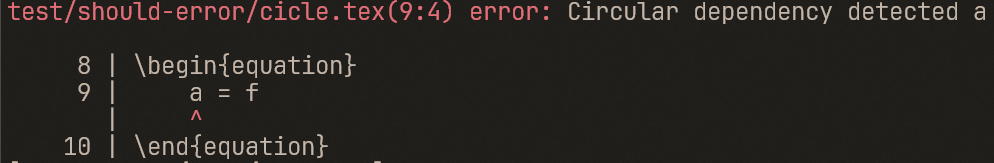
\includegraphics[scale=0.5]{./Imagens/error-circular-deps.png}
    \end{center}
\end{figure}


\subsection{Inferência de Tipos} \label{subsection-type-inference}


A função \verb`infer_type` determina o tipo de uma expressão (\verb`expr`) na AST durante a análise semântica, aplicando regras baseadas em operações matemáticas, como multiplicação entre número real e vetor, produto vetorial entre vetores e assinaturas de funções. 

Projetada para processar todas as expressões de \texttt{EquationLang} — como identificadores, operadores, chamadas de função e literais —, a função verifica inicialmente se o tipo já foi inferido (\verb"expr.ty_inferred") para evitar processamento redundante. Caso contrário, realiza a inferência com base em um \verb"switch" que é capaz de avaliar todos tipos de expressões. Um trecho relevante desse processo está no \autoref{cod-type-inference}, que ilustra a discriminação e validação dos tipos.

Para \textbf{identificadores} (\verb"Expr_Identifier"), verifica se o identificador corresponde a um vetor especial, como $\omega_i$ ou $\vec{n}$. Nesse caso, o tipo é inferido como $\mathbb{R}^3$ (vetor tridimensional). Identificadores específicos, como \verb"\pi" ou \verb"\epsilon", são atribuídos ao tipo numérico real ($\mathbb{R}$). Para outros identificadores, a função consulta o escopo atual para determinar o tipo, usando as estruturas detalhado na \autoref{section-escope-table}.

\begin{codigo}[htb]
    \caption{\small Parte do switch da inferencia de tipos. }
    \label{cod-type-inference}
\begin{lstlisting}[language=C, frame=none, inputencoding=utf8]
infer_type :: proc(expr: ^ast.Expr, allow_invalid := false, default : ^ast.Type = ast.ty_invalid ) -> ^Type {
    /// Código omitido por brevidade  ///
    #partial switch e in expr.derived {
    case ^Expr_Identifier:
        // Alway set by the parser if indentifier starts with `\vec{}`
        if e.is_vector {
            type = new_type_vector(ty_number, 3) // vector 3 of type number (real)
        } else if e.identifier.kind == .Pi || e.identifier.kind == .Epsilon {
            type = ty_number
        } else {
            key := key_from_identifier(e)
            sym, ok := scope_get(key)
            if ok {
                if sym.type != nil {
                    type = sym.type
                }
            }
            /// Código omitido por brevidade  ///
        }

    case ^Expr_Prefix:
        right_type := infer_type(e.right, allow_invalid, default)
        /// Código omitido, mas aqui fazemos a validação da subexpressão direita e atribuimos o tipo correto para Expr_Prefix   ///

    case ^Expr_Infix:
        ty_left  := infer_type(e.left, allow_invalid, default)
        ty_right := infer_type(e.right, allow_invalid, default)
        /// Código omitido
        //  Inferimos tipo da expressão esquerda e direto dessa operação binária
        //  Depois validamos compatibilidade considerando a operação sendo usada nessas duas expressões

    /// Outros casos ...  ///
}
\end{lstlisting}
\end{codigo}


Para \textbf{operações prefixadas} (\verb"Expr_Prefix"), como raiz quadrada (\verb"\sqrt") ou funções trigonométricas (\verb"\sin", \verb"\cos"), a função valida se o operando é numérico e atribui o tipo correspondente à expressão. Nas \textbf{operações binárias} (\verb"Expr_Infix"), a função realiza a inferência dos tipos dos operandos esquerdo e direito. Se os tipos não forem compatíveis, aplica regras específicas. Alguma dessas regras são:

\begin{itemize}
    \item A multiplicação de um número por um vetor ($2*\vec{n}$) ou a divisão de um vetor por um número ($\frac{\vec{u}}{\sqrt{\vec{u} \cdot \vec{u}}}$) resultam no tipo vetor ($\mathbb{R}^3$).
    \item Operações entre dois números resultam em um número.
    \item Operações entre dois vetores resultam em um número ou um vetor a depender se a operação foi um produto vetorial ou produto interno.
\end{itemize}

Outros casos incluem \textbf{literais}, como números (\verb"Expr_Number") e vetores literais \\(\verb"Expr_Vector_Literal"), cujos tipos são atribuídos diretamente como $\mathbb{R}$ (números reais) e $\mathbb{R}^3$ (vetores tridimensionais), respectivamente.



Para chamadas de função (\verb"Expr_Function_Call"), o tipo da expressão é determinado pelo tipo do primeiro valor retornado pela função. A validação dos argumentos é realizada em outra função, detalhada na \autoref{subsubsection-eq-func-defn}. % ; Essa parte já foi dita
% Além disso, a função realiza validações específicas para evitar inconsistências, como garantir que operações entre vetores sejam semanticamente válidas (e.g., divisão entre vetores não é permitida). 

% Em resumo, \verb`infer_type` é uma implementação robusta e flexível de inferência de tipos, essencial para a análise semântica de um compilador. A função assegura que cada expressão receba um tipo coerente com a semântica da linguagem, lidando com uma ampla gama de construções sintáticas e oferecendo suporte extensível para futuras adições à linguagem.

\subsection{Validação de Equações}

As declarações de equações são validadas após a coleta e ordenação descritas na \autoref{subsection-sym-resolution}, portanto assume-se que o lado esquerdo das equações seja um identificador válido ou uma definição de função e que estão na ordem correta de avaliação.

Qualquer violação semântica, como incompatibilidades de tipos ou uso de escalares onde vetores são esperados, é reportada ao usuário, com detalhes sobre o contexto e a localização do erro, conforme descrito em \autoref{subsection-erros}.

A função \verb"check_expr" realiza uma travessia semelhante à inferência de tipos e chama \texttt{infer\_type}. Nela, a análise de expressões que não foram abordadas por \texttt{infer\_type} é realizada para todos os tipos de expressões. Algumas dessas validações estão listadas após este parágrafo, e um trecho dessa travessia pode ser visto no \autoref{eq-function-check-expr}.

\begin{itemize}
    \item \verb`Expr_Function_Call`: Verifica se estamos fazendo a chamada corretamente com um identificador, evitando casos como tentar chamar uma função com um número, por exemplo, $123(x,y)$, o que é incorreto. Também checa se o número de argumentos corresponde ao número de parâmetros esperados.
    \item \verb`Expr_Prefix`: Verifica operadores (\verb`-`, \verb`+`) e funções como \verb`sqrt(x)` e \verb`sin(x)`. Certifica-se de que os tipos sejam compatíveis, gerando erro em caso contrário, como quando um vetor é passado para a função seno.
    \item Literais de Vetor \verb`Expr_Vector_Literal`: Garante que os vetores tenham exatamente 3 dimensões\footnote{Exigir vetores de apenas 3 dimensões pode ser considerado uma limitação semântica imposta pelo compilador}.
\end{itemize}




\begin{codigo}[H]
    \caption{\small Identificadores embutidos pela convenção deste trabalho.}
    \label{cod-builtins}
\begin{lstlisting}[language=C, numbers=none, frame=none, inputencoding=latin1]
BUILTIN_IDENTIFIERS :: []string {
    `\pi`,
    `\epsilon`,
    `\theta{h}`,
    `\vec{n}`,
    `\vec{h}`,
    `\vec{\omega{i}}`,
    `\theta{i}`,
    `\phi{i}`,
    `\vec{\omega{o}}`,
    `\theta{o}`,
    `\phi{o}`,
    `\theta{h}`,
    `\theta{d}`,
}
\end{lstlisting}
\end{codigo}


\begin{codigo}[H]
    \caption{\small Recorte da função \texttt{check\_expr}. }
    \label{eq-function-check-expr}
\begin{lstlisting}[language=C, basicstyle=\ttfamily\footnotesize, frame=none, inputencoding=utf8]
check_expr :: proc(expr: ^ast.Expr) {
    // Primeiro inferimos o tipo
    infer_type(expr)
    // Código omitido de preambulo
        case ^Expr_Identifier:
            // Check for using undefined indetifiers
            identifier_key := key_from_identifier(e)
            if !is_defined(e, false) {
                error(e.identifier,  "Identifier `%v` is not defined in the current scope.", identifier_key)
            }
        case ^Expr_Function_Call:
            check_expr(e.left)
            fn_ident, fn_ident_ok := e.left.expr_derived.(^ast.Expr_Identifier)
            if !fn_ident_ok {
                error(e.open,  "Tried to call an expression that is not an identifier")
            }
            fn_string := key_from_identifier(fn_ident)
            fn_sym, fn_sym_ok := scope_get(fn_string)
            fn_type, fn_type_ok := e.left.ty_inferred.derived.(^ast.Type_Function)
            if !fn_type_ok {
                error(e.open,  "Tried to call`%v`, which is not a function. Its type is `%v`", fn_string, format_type(e.left.ty_inferred))
            }
            if len(e.exprs) != len(fn_type.params) {
                error(
                    e.open,  "Args number mismatch. `%v` function expects  `%v` arguments but `%v` were given.",
                    fn_string, len(fn_type.params), len(e.exprs)
                )
            }
        // Outros casos omitidos
    }
}

\end{lstlisting}
\end{codigo}



\subsection{Validação de Funções}
A validação semântica de definições e chamadas de funções segue um processo semelhante ao da análise de expressões, mas com o uso da pilha de escopos.
Nas definições de funções, as variáveis no corpo da função são validadas para assegurar que todos os símbolos usados realmente estejam definidos no escopo da função. Já nas chamadas de funções, os argumentos fornecidos são comparados aos parâmetros esperados para validação.

\subsubsection{Definição de Funções} \label{subsubsection-eq-func-defn}

O procedimento \verb"check_function_definition" valida definições de funções, garantindo segurança de tipos e consistência através das seguintes tarefas:

\begin{enumerate}
    \item Inferir os tipos dos parâmetros.
    \item Inferir o tipo de retorno baseado na expressão final.
    \item Construir o tipo completo da função, incluindo parâmetros e retorno.
    \item Garantir que os identificadores usados estejam consistentes com seus tipos declarados.
    \item Validar as expressões no corpo da função.
    \item Criar um novo escopo para os parâmetros da função.
\end{enumerate}

O processo começa com o processamento dos parâmetros e o gerenciamento do escopo, como mostrado no \autoref{cod-parametros-validation}. Quando uma função é definida, um novo escopo é criado para armazenar informações dos parâmetros e da função, que são adicionadas ao escopo correspondente.

Esse escopo é essencial para validar chamadas de função e expressões no corpo. Cada função tem seu próprio escopo, com o escopo pai sendo o global, evitando conflitos de identificadores.

O controle de visibilidade funciona como esperado; se um parâmetro $x$ existe, ele é preferido ao $x$ global, resultando no fenômeno de \textit{shadowing} ou sombreamento, como exemplificado na \autoref{eq-shadowing}, onde o valor de $f$ é 3, não 2.

\begin{align} \label{eq-shadowing}
    &x = 2 \\
    &g(x) = x \\
    &f = g(3)
\end{align}


Durante a validação dos parâmetros, cada identificador passa por um processo de inferência de tipo. Parâmetros marcados explicitamente com o prefixo \verb"\vec" recebem o tipo padrão $\mathbb{R}^3$ (vetor tridimensional), enquanto os demais são tratados como número real ($\mathbb{R}$).

Se um parâmetro $\vec{x}$ é declarado como vetor, todas as operações envolvendo $x$ no corpo da função devem respeitar as operações vetoriais; caso contrário, um erro será reportado.

\subsubsection{Chamada de Funções}
Chamadas de função passam por uma validação semelhante: os argumentos têm seus tipos inferidos e são comparados com a assinatura da função chamada (\verb"Type_Function").

No exemplo do \autoref{cod-type-mismatch}, a função $g$ possui a assinatura $\mathbb{R} \times \mathbb{R} \to \mathbb{R}$. A expressão resultante da chamada de função terá o tipo do contradomínio da função. Também é necessário confirmar que $g$ refere-se a um símbolo do tipo função.

\begin{codigo}[H]
    \caption{\small Equação com uso incorreto de tipos na chamada de função.}
    \label{cod-type-mismatch}
\begin{lstlisting}[language=tex, numbers=none, frame=none, inputencoding=latin1]
\begin{equation}
    g(a, x) = a*x*x
\end{equation}

\begin{equation}
    f = g(1, \vec{1,1,1})
\end{equation}

\end{lstlisting}
\end{codigo}

A função $g$ espera dois números reais como argumentos, mas na equação $f$, um vetor foi passado no lugar de um número, o que gera um erro. A \autoref{fig-type-mismatch} ilustra esse erro, indicando a função com o argumento incompatível. Além disso, ao passar os argumentos, também validamos se a quantidade de argumentos corresponde ao número de parâmetros esperados.

\begin{figure}[H]
    \caption{\label{fig-type-mismatch} \small Erro gerado por uso incorreto de tipos na chamada de função.}
    \begin{center}
        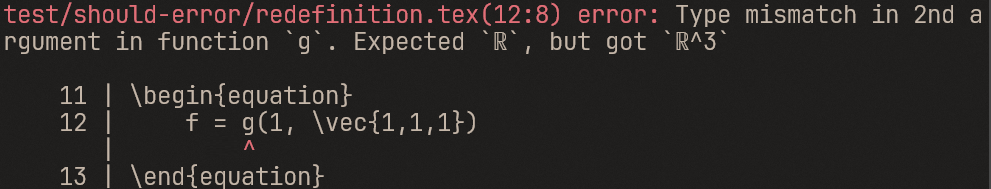
\includegraphics[scale=0.5]{./Imagens/error-type-mismatch.png}
    \end{center}
\end{figure}


\begin{codigo}[H]
    \caption{\small Validação de parâmetros de uma função.}
    \label{cod-parametros-validation}
\begin{lstlisting}[language=C, numbers=none, frame=none, inputencoding=latin1]
// ...
parameter_types := [dynamic]^Type{}
scope_enter(fn_sym.scope) {
    for &parameter in fn.parameters {
        parameter_key := key_from_identifier(parameter)
        ty := infer_type(parameter, true, ty_number)
        parameter_sym.type = ty
        append(&parameter_types, ty)
    }
}
// ...
\end{lstlisting}
\end{codigo}

%
% \begin{codigo}[htb]
%     \caption{\small Gerenciamento de escopo na validação do corpo da função.}
%     \label{cod-scope-management}
% \begin{lstlisting}[language=C, numbers=none, frame=none, inputencoding=latin1]
% scope_enter(fn_sym.scope) {
%     // Validação do corpo da função
%     check_expr(body)
%     // Inferência e validação de tipo
%     body_type := infer_type(body)
% }
% \end{lstlisting}
% \end{codigo}

%
% \begin{codigo}[htb]
%     \caption{\small .}
%     \label{cod-types-structs}
% \begin{lstlisting}[language=C, numbers=none, frame=none, inputencoding=utf8]
% case ^Decl_Equation:
%     check_decl(s)
%
% scope_enter(fn_sym.scope) {
%     // Validação do corpo da função
%     check_expr(body)
%     // Inferência e validação de tipo
%     body_type := infer_type(body)
%     result_types := [dynamic]^Type{body_type}
%     fn_type := make_function_type(parameter_types[:], result_types[:])
% }
% \end{lstlisting}
% \end{codigo}



\section{Geração de Código (\texttt{emitter})} \label{section-emitter}


A etapa de geração de código é realizada pelo pacote \texttt{emitter}, que cria um \textit{shader} compatível com a ferramenta Disney BRDF Explorer. Essa etapa é separada em três fases, descrita na \autoref{sub-start-emitting}. O processo começa com o escopo global, que contém informações essenciais, como símbolos, assinaturas de funções, tipos e nós da AST completamente anotada. A travessia recursiva dos símbolos e nós ocorre sem validações adicionais, uma vez que a etapa semântica já foi realizada.

A geração de código abrange o lado esquerdo da equação, que inclui identificadores e parâmetros de funções, e o lado direito, que é sempre uma expressão, cuja emissão é explorada em \autoref{sec-RHS}. Além disso, é fundamental garantir que cada variável tenha um nome único no código GLSL, conforme descrito em \autoref{sec-unicidade}.

\subsection{Emissão de Equações} \label{subsection-emission}

A emissão de código começa pelo lado esquerdo da equação. Existem três aspectos principais nesse processo:
\begin{enumerate}
    \item Mapeamento de Tipos: O tipo associado ao identificador é a primeira informação a ser resolvida. Caso seja um número real, ele é mapeado para \verb"float" em GLSL. Para vetores ($\mathbb{R}^3$), o mapeamento é feito para \verb"vec3". Em definições de funções, a assinatura é construída com base nos tipos dos parâmetros e do retorno.

    \item Identificado: O identificador associado ao símbolo é traduzido conforme regras específicas que garantem unicidade e conformidade com as restrições do GLSL. Este processo é detalhado em \autoref{sec-unicidade}.

    \item Expressões: No caso do lado direito da equação, tanto funções quanto de variaveis, são expressões. Para gerar isso, realiza-se uma travessia da AST, mapeando nós de expressões (como somas e chamadas de funções trigonométricas) para seu equivalente em GLSL. Detalhes adicionais sobre a emissão de código para expressões estão na \autoref{sec-RHS}.
\end{enumerate}



\subsection{Unicidade de Variáveis} \label{sec-unicidade}

Para garantir unicidade e compatibilidade dos identificadores gerados no GLSL, é necessário lidar com algumas restrições sintáticas e evitar colisões entre identificadores.

\begin{enumerate}
    \item \textbf{Restrição de Caracteres}: O GLSL não permite caracteres especiais, como \verb"{" e \verb"}", em seus identificadores. Por exemplo, uma equação em \texttt{EquationLang} \verb "f_{1} = 2" não pode ser diretamente transformada no identificador \verb`f_{1}`. Para resolver isso, todos os caracteres inválidos são substituídos por sublinhados (\verb`_`), considerando subexpressões, resultando em identificadores como \verb`f__1_`.

    \item \textbf{Prevenção de Colisões}: Mesmo após a substituição de caracteres, podem ocorrer colisões. Para resolver isso, mapeia-se cada a simbolo de identificador cada para um inteiro único de 64 bits (ID). Esse ID é então concatenado ao começo desse identificador com o prefixo \verb`var`, resultando em \verb`var1_f__1_`; uma cadeia de carateres unica para simbolo.

    \item \textbf{Remoção de Sequências Reservadas}: O GLSL reserva identificadores que contêm duas ou mais ocorrências consecutivas de \verb`_`, Também é necessário remover sublinhados ao final, resultando em \verb`var1_f_1`. Após a geração inicial, identificadores que contenham essas sequências são corrigidos para atender às restrições do GLSL, resultado.
\end{enumerate}


Essas etapas garantem que cada variável no código GLSL seja única e válida. Apesar da limitação de $2^{64} - 1$ identificadores distintos imposta pelo uso de inteiros de 64 bits, esse valor é mais do que suficiente para o propósito de criação de BRDFs. Caso necessário, a utilização de inteiros de tamanho arbitrário implementado por \textit{software} para ampliar esse limite.

%%%%%%%


\subsection{Geração de Expressões} \label{sec-RHS}

A geração de expressões no pacote \texttt{emitter} converte as expressões do lado direito das equações em código GLSL válido, usando a AST anotada com tipos inferidos.

A função principal, \verb"emit_expr", processa cada nó de expressão e constrói a cadeira de caracteres correspondente em GLSL usando um \verb"StringBuilder" da biblioteca padrão de Odin, evitando concatenações excessivas. Na travessia recursiva da AST, realizada pelo pacote \texttt{walker}, converte operações binárias, prefixas, vetoriais e chamadas de função em código \textit{shading}.

Um trecho dessa função está no \autoref{cod-emit-expr}, que demonstra como os tipos são discriminados (\texttt{case}) e \textit{string}s\footnote{string é uma cadeia de caracteres} para funções trigonométricas são geradas usando \verb|sbprint|. A seguir, são enumeradas as principais categorias de expressões tratadas:

\begin{enumerate}
    \item \textbf{Expressões Prefixas (\texttt{Expr\_Prefix})}:
    Essas expressões incluem operações unárias e funções matemáticas básicas. A implementação:
    \begin{itemize}
        \item Emite funções trigonométricas através dão funlão providas por GLSL autometicamente, como \verb|sin|, \verb|cos| e \verb|tan|.
        \item Lida com operadores unários, como negação (\verb|-|) e raiz quadrada (\verb|sqrt|). Nesses casos é aplicar escrever o operador com parentesis ao redor. Por exemplo, \verb"\sqrt{-2}" ($\sqrt{-2}$) emite \verb"(sqrt(-(2)))".
        \item Constrói vetores usando o construtor provido por OpenGL \verb|vec3()|.
        \item Mantém a precedência de operadores adicionando parênteses apropriados.
    \end{itemize}

    \item \textbf{Expressões Binárias (\texttt{Expr\_Infix})}:
    Operações binárias representam a maior parte das expressões matemáticas.
    \begin{itemize}
        \item Operações aritméticas básicas (\verb|+|, \verb|-|, \verb|*|, \verb|/|), basta adionar parenteses com o operador no meio, e emitir a esquerda e direita recursivamente.
        \item Produto interno, usa-se função \verb|dot| provida por GLSL.
        \item Multiplicação escalar-vetor é suportado por GLSL, então fica similair ao original \verb"\vec{n} \cdot 2" equivalente à \verb"(vec3(n)*2)".
        \item Suporta o produto vetorial (\verb|cross|). Nesse caso o operador vem primeiro, no lugar de infixo, \verb"\vec{n_1} \\ \cross $\vec{n_2}$" equivalente à  \\ \verb"cross(vec3(var_1_n_1),vec3(var_2_n_2))".
        \item Processa exponenciação (\verb|x^y|) chamando a função \verb|pow()| do GLSL.
    \end{itemize}

    \item \textbf{Expressões Literais e Agrupamentos}:
    \begin{itemize}
        \item Constrói vetores literais utilizando \verb|vec3|.
        \item Adicionar parênteses em expressões agrupadas.
    \end{itemize}

    \item \textbf{Expressões de Chamadas de Função}:
       Na geração de uma chamada de função, ocorre a chamada recursiva para emitir a expressão do identificador dessa função. Em seguida, abre-se um parêntese \verb"(", emite-se uma expressão para cada argumento, separados por vírgula, e, por fim, fecha-se o parêntese. Isso é demonstrado pelo trecho no \autoref{cod-emission-func}.

\end{enumerate}

\begin{codigo}[htb]
    \caption{\small Emissão de chamada de funções. }
    \label{cod-emission-func}
\begin{lstlisting}[language=C, frame=none, inputencoding=utf8]

        case ^Expr_Function_Call:
        emit_expr(sb, e.left)
        sbprint(sb, '(')
        for arg, idx in e.exprs {
            emit_expr(sb, arg)
            if idx < (len(e.exprs) -1)  {
                sbprint(sb, ',')
            }
        }
        sbprint(sb, ')')
\end{lstlisting}
\end{codigo}


 Esse sistema permite traduzir expressões matemáticas como mostrada na \autoref{eq-emit-expr-example}, gerando o código correspondente apresentado no \autoref{cod-emit-expr-example}.

\begin{subequations}
    \label{eq-emit-expr-example}
\begin{equation}
    \rho_{d} = \vec{0,1,1}
\end{equation}

\begin{equation}
    \rho_{s} = \vec{1,0,1}
\end{equation}

\begin{equation}
    n = +2^8
\end{equation}

\begin{equation}
f = \frac{\rho_{d}}{\pi} + \rho_{s} * \frac{n+2}{2*\pi} *
\cos{\theta_{h}}^{n}
\end{equation}
\end{subequations}

\begin{codigo}[htb]
   \caption{\small Exemplo de código de expressão gerado. }
   \label{cod-emit-expr-example}
\begin{lstlisting}[language=C, frame=none, inputencoding=utf8]
  var_12_rho_d = vec3(0.0, 1.0, 1.0);
  var_13_n     = pow(2.0, 8.0);
  var_14_rho_s = vec3(1.0, 0.0, 1.0);
  var_15_f     = ((var_12_rho_d / var_1_pi) +
              ((var_14_rho_s * ((var_13_n + 2.0) / (2.0 * var_1_pi))) *
               pow(cos(var_10_theta_h), var_13_n)));
\end{lstlisting}
\end{codigo}

\begin{codigo}[htb]
   \caption{\small Emitir expressão. }
   \label{cod-emit-expr}
\begin{lstlisting}[language=C, basicstyle=\ttfamily\footnotesize, frame=none, inputencoding=utf8]
    case ^Expr_Prefix:
        #partial switch e.op.kind {
        case .ArcSin:
            sbprint(sb, "asin(")
            emit_expr(sb, e.right)
            sbprint(sb, ")")
            return

        //... Outros casos omissos

        case .Tan:
            sbprint(sb, "tan(")
            emit_expr(sb, e.right)
            sbprint(sb, ")")
            return
        case .Exp:
            sbprint(sb, "exp(")
            emit_expr(sb, e.right)
            sbprint(sb, ")")
            return
        case .Vec:
            ty_vec, ok := e.ty_inferred.derived.(^ast.Type_Vector)
            assert(ok && ty_vec.dimensions == 3)

            sbprint(sb, "vec3(")
            emit_expr(sb, e.right)
            sbprint(sb, ")")
            return
    case ^Expr_Infix:
        op: string
        #partial switch e.op.kind {
        case .Plus:  op = "+"
        case .Minus: op = "-"
        case .Mul:
            // Check if both operands are vectors
            if is_vector(e.left.ty_inferred) && is_vector(e.right.ty_inferred) {
                sbprint(sb, "dot(")
                emit_expr(sb, e.left)
                sbprint(sb, ",")
                emit_expr(sb, e.right)
                sbprint(sb, ")")
                return
            } else {
                op = "*"
            }
        case .Frac, .Div:  op = "/"
        // Especially handled because it's not infix in glsl
        case .Caret: op = ""
            sbprint(sb, "pow(")
            emit_expr(sb, e.left)
            sbprint(sb, ",")
            emit_expr(sb, e.right)
            sbprint(sb, ")")
            return

        //... Outros casos omissos
        case .Cross: op = ""
            sbprint(sb, "cross(")
            emit_expr(sb, e.left)
            sbprint(sb, ",")
            emit_expr(sb, e.right)
            sbprint(sb, ")")
            return

        sbprint(sb, '(')
        emit_expr(sb, e.left)
        sbprint(sb, op)
        emit_expr(sb, e.right)
        sbprint(sb, ')')


   //... 

\end{lstlisting}
\end{codigo}

\subsection{Fases do Processo de Geração do Shader}
\label{sub-start-emitting}

A função \verb"emit" é o ponto de partida do processo de emissão de código, onde ocorre a transformação final da AST em um shader GLSL. Este processo é dividido em três fases principais, cada uma com responsabilidades bem definidas para garantir a geração correta do código.

\begin{enumerate}
    \item \textbf{Inicialização e Estruturação} \\
    Nesta etapa inicial, o foco está em estabelecer a base do shader GLSL. Isso inclui:
    \begin{itemize}
        \item \textbf{Parâmetros}: Emissão de uma seção parametrizável, \verb"::begin parameters ::end parameters", dos shaders, requerida pela ferramenta Disney BRDF Explorer.
        \item \textbf{Marcadores de Seção}: Adição de delimitadores como \verb|::begin shader| e \verb|::end shader|, que iniciam o código GLSL na ferramenta da Disney.
        \item \textbf{Built-in}s: Emissão das declarações e definições de variáveis e funções \textit{built-in} necessárias, para dar ao shader suporte às convenções da \autoref{tab-conventions-metodologia}.
    \end{itemize}

    \item \textbf{Processamento de Símbolos} \\
    Após a estruturação inicial, a função processa uma tabela de símbolos (\verb|Scope|) para organizar as declarações e definições necessárias. As operações nesta fase incluem:
    \begin{itemize}
        \item \textbf{Iteração sobre Símbolos}: Processamento de variáveis escalares (\verb|Type_Basic|), definições de funções (\verb|Type_Function|) e variáveis vetoriais (\verb|Type_Vector|).
        \item \textbf{Separação de Declarações e Definições}: Uso de duas instâncias distintas de \texttt{StringBuilder}, uma para declarações, que devem vir antes para que as variáveis possam ser usadas globalmente, e outra para definições que podem fazer uso dessas declarações sejam built-ins ou definidos pelos usuários.
    \end{itemize}

    \item \textbf{Emissão Final} \\
    A fase final concatena os elementos gerados anteriormente, garantindo que o código esteja na ordem correta para compilação. Essa fase gera a função principal \verb|BRDF|, que contém todas as declarações concatenadas, somadas às declarações e preâmbulos. Por fim, é realizada a gravação em disco do shader completo.
\end{enumerate}


\subsubsection{Variáveis Built-in}
A emissão correta de um shader de BRDF necessita da geração de variáveis \textit{built-in} diretamente no \textit{shader}, conforme ilustrado na \autoref{cod-builtins-emitted}. Essas variáveis, presentes na tabela \autoref{tab-conventions}, seguem as convenções estabelecidas e são inicializadas automaticamente dentro da função de entrada do \textit{shader}, denominada \verb|BRDF|, conforme o padrão da ferramenta Disney.

Essas variáveis fornecem a infraestrutura necessária para cálculos de reflectância bidirecional em shaders GLSL. A ferramenta Disney disponibiliza algumas delas como parâmetros da função de entrada \verb`BRDF`, mas com nomenclaturas diferentes das adotadas neste trabalho. Essas parametros são: \verb"N" que representa a normal da superfície; \verb"L" que indica a direção da luz incidente (L); \verb"V" que representa a direção de visualização. As demais variáveis são calculadas na emissão de código.

Para calcular variáveis como \verb`omega_i`, \verb`theta_d` e \verb`phi_i`, foram desenvolvidas funções auxiliares que produzem strings válidas em GLSL. A entrada dessas funções é uma \textit{string} representando o vetor (\verb`v`), substituída diretamente no corpo do GLSL gerado:
\begin{itemize}
    \item \verb`phi(v)`: Calcula o ângulo azimutal ($\phi$), gera \verb`atan(sqrt(v.y*v.y + v.x*v.x), v.z)`.
    \item \verb`theta(v)`: Calcula o ângulo polar ($\theta$) com a expressão \verb`atan(v.y, v.x)`.
\end{itemize}

A declaração dessas variáveis embutidas é realizada pela função \\ \verb`emit_builtin_globals_declaration`, que também define constantes matemáticas como \verb`\pi`  e \verb`\epsilon`. É apresentado na \autoref{tab-conventions} como cada convenção é mapeada para código GLSL. Para maior clareza, o prefixo das variáveis discutido na seção de unicidade (\autoref{sec-unicidade}) foi removido.

\begin{table}[h]
    \centering
    % \begin{tabular}{|c|l|}
    \begin{tabular}{c|l}
        \hline
        \textbf{Símbolo} & \textbf{Código GLSL Gerado} \\
        \hline
        $\theta_i$ & \verb"atan(omega_i.y, omega_i.x)" \\
        \hline
        $\theta_o$ & \verb"atan(omega_o.y, omega_o.x")\\
        \hline
        $\phi_i$ & \verb"atan(sqrt(omega_i.y*omega_i.y+omega_i.x*omega_i.x),omega_i.z)" \\
        \hline
        $\phi_o$ & \verb"atan(sqrt(omega_o.y*omega_o.y+omega_o.x*omega_o.x),omega_o.z")\\
        \hline
        $\omega_i$ & \verb"L " \\
        \hline
        $\omega_o$ & \verb"V " \\
        \hline
        $\vec{n}$ & \verb"normalize(N)" \\
        \hline
        $\vec{h}$ & \verb"normalize(L+V")\\
        \hline
        $\theta_h$ & \verb"acos(dot(vec_h , vec_n))" \\
        \hline
        $\theta_d$ & \verb"acos(dot(vec_h , omega_i))" \\
        \hline
        $\pi$ & \verb"3.141592653589793" \\
        \hline
        $\epsilon$ & \verb"1.192092896e-07" \\
        \hline
    \end{tabular}
    \caption{Tabela de mapeamento de conveções para código GLSL}
    \label{tab-conventions}
\end{table}

% Este sistema fornece uma base suficiente para implementação de BRDFs complexas.

\begin{codigo}[htb]
    \caption{\small Recorte da função BRDF one as variaveis built-ins são inicializadas }
    \label{cod-builtins-emitted}
\begin{lstlisting}[language=C, frame=none, inputencoding=utf8]
  //////////// START OF BUILTINS INITIALIZATION ////////////
  var_0_vec_h = normalize(L + V);
  var_3_vec_n = normalize(N);
  var_1_pi = 3.141592653589793;
  var_2_epsilon = 1.192092896e-07;
  var_4_vec_omega_i = L;
  var_5_theta_i = atan(var_4_vec_omega_i.y, var_4_vec_omega_i.x);
  var_6_phi_i = atan(sqrt(var_4_vec_omega_i.y * var_4_vec_omega_i.y +
                          var_4_vec_omega_i.x * var_4_vec_omega_i.x),
                     var_4_vec_omega_i.z);
  var_7_vec_omega_o = V;
  var_8_theta_o = atan(var_7_vec_omega_o.y, var_7_vec_omega_o.x);
  var_9_phi_o = atan(sqrt(var_7_vec_omega_o.y * var_7_vec_omega_o.y +
                          var_7_vec_omega_o.x * var_7_vec_omega_o.x),
                     var_7_vec_omega_o.z);
  var_10_theta_h = acos(dot(var_0_vec_h, N));
  var_11_theta_d = acos(dot(var_0_vec_h, var_4_vec_omega_i));
  //////////// END OF BUILTINS INITIALIZATION ////////////
\end{lstlisting}
\end{codigo}




% ---------
%
% Nos resultados eu falo mais XD emissão
%
% Uma coisa imporatnte a se dizer é todas em EquationLang todas as equações podem ser referenciadas em ourtas equações para isso pode ser possivel em GLSL, declarações todas as variaveis primeiro fora da função BRDF, efetivamente deixando-as globais. E só ao entrar na função é que inicializados, isso vale para as variaveis embutidas tbm \autoref{cod-builtins}. Isso é feito principalmente para deixar as variaveis visiveis dentro um função em GLSL assim como semanticamente é possivel em EquationLang. @Diga pra nota em agluma imagem mostrando isso@ Outra coisa é que todas as equaqações estão na ordem correta de avaliação já que isso foi feito através da ordernação topológica feita anteriormente, então as decalarções globais são cosistente, sempre, e vão conseguir rodar no GLSL @informal@.

\subsection{Emissão de Definições de Função}

A emissão de definições de função ocorre antes da inicialização das variáveis. A assinatura da função, que inclui o nome (baseado na estratégia da \autoref{sec-unicidade}), é gerada, juntamente com o tipo de retorno e os parâmetros, mapeados conforme a \autoref{subsection-emission}. Os nomes dos parâmetros são determinados pelos símbolos presentes no escopo da função, enquanto o corpo da função é emitido chamando \verb|emit_expr|, da mesma forma que a emissão de expressões.

O mapeamento entre tipos em \texttt{EquationLang} e GLSL é bijetivo, garantindo que qualquer função definida em \texttt{EquationLang} possa ser representada em GLSL. Um exemplo de definição gerada é mostrado na \autoref{cod-normalize-reflect}, que se refere às funções de reflexão e normalização da equação \autoref{eq-normalize-reflect}. Os nomes gerados seguem a numeração discutida na \autoref{sec-unicidade}, e o retorno é sempre avaliado como uma única expressão.


\label{eq-normalize-reflect} \begin{subequations}
\begin{equation}
  \text{normalize}(\vec{u}) = \frac{\vec{u}}{\sqrt{\vec{u} \cdot \vec{u}}}
\end{equation}

\begin{equation}
reflect(\vec I, \vec N) =  2*(\vec I \cdot \vec N)*\vec N - \vec I
\end{equation}
\end{subequations}

\begin{codigo}[htb]
   \caption{\small Código GLSL gerado pelo compilador para as funções de normalização e reflexão de vetores. }
   \label{cod-normalize-reflect}
\begin{lstlisting}[language=C, inputencoding=utf8]
//////////// START FUNCTIONS DECLARATIONS ////////////
vec3 var_13_reflect(vec3 var_14_vec_I, vec3 var_15_vec_N) {
    return (((2.0*(dot(var_14_vec_I,var_15_vec_N)))*var_15_vec_N)-var_14_vec_I);
}

vec3 var_17_text_normalize(vec3 var_18_vec_u) {
    return (var_18_vec_u/sqrt(dot(var_18_vec_u,var_18_vec_u)));
}
//////////// END FUNCTIONS DECLARATIONS ////////////

\end{lstlisting}
\end{codigo}

